\documentclass[12pt]{book}
\usepackage[width=4.375in, height=7.0in, top=1.0in, papersize={5.5in,8.5in}]{geometry}
%\usepackage[pdftex]{graphicx}
\usepackage{amsmath}
\usepackage{amssymb}
\usepackage{tipa}
%for using the euro sign
\usepackage{eurosym}
\usepackage{graphicx}
%\usepackage{txfonts}
\usepackage{textcomp}
%\usepackage{amsthm}
\usepackage{array}
%\usepackage{xy}
\usepackage{fancyhdr}

\usepackage{hyperref}

%Ommit some vbox and hbox errors (under 10000)
\vbadness=10000
\hbadness=10000

%The below is used for codes
\usepackage{color}

\definecolor{dkgreen}{rgb}{0,0.6,0}
\definecolor{gray}{rgb}{0.75,0.75,0.75}
\definecolor{mauve}{rgb}{0.58,0,0.82}
\usepackage{listings}
\lstset{
  backgroundcolor=\color{gray},  % choose the background color; you must add \usepackage{color} or \usepackage{xcolor}
  basicstyle=\footnotesize,       % the size of the fonts that are used for the code
  breakatwhitespace=false,        % sets if automatic breaks should only happen at whitespace
  breaklines=true,                % sets automatic line breaking
  captionpos=b,                   % sets the caption-position to bottom
  commentstyle=\color{dkgreen},   % comment style
  deletekeywords={...},           % if you want to delete keywords from the given language
  escapeinside={@}{@)},         % if you want to add LaTeX within your code
  %extendedchar=true,              % lets you use non-ASCII characters; for 8-bits encodings only, does not work with UTF-8
  frame=single,                   % adds a frame around the code
  keywordstyle=\color{mauve},      % keyword style
  language=C,                % the language of the code
  morekeywords={*,...},           % if you want to add more keywords to the set
  numbers=left,                   % where to put the line-numbers; possible values are (none, left, right)
  numbersep=5pt,                  % how far the line-numbers are from the code
  numberstyle=\tiny\color{dkgreen},  % the style that is used for the line-numbers
  rulecolor=\color{black},        % if not set, the frame-color may be changed on line-breaks within not-black text (e.g. comments (green here))
  showspaces=false,               % show spaces everywhere adding particular underscores; it overrides 'showstringspaces'
  showstringspaces=false,         % underline spaces within strings only
  showtabs=false,                 % show tabs within strings adding particular underscores
  stepnumber=1,                   % the step between two line-numbers. If it's 1, each line will be numbered
  stringstyle=\color{mauve},      % string literal style
  tabsize=4,                      % sets default tabsize to 2 spaces
  title=\lstname,                  % show the filename of files included with \lstinputlisting; also try caption instead of title
}
%until here

\newcommand{\tab}{\hspace*{2em}}


\pagestyle{fancy}
\renewcommand{\chaptermark}[1]{\markboth{#1}{}}
\renewcommand{\sectionmark}[1]{\markright{\thesection\ #1}}
\fancyhf{}
\fancyhead[LE,RO]{\bfseries\thepage}
\fancyhead[LO]{\bfseries\rightmark}
\fancyhead[RE]{\bfseries\leftmark}
\renewcommand{\headrulewidth}{0.5pt}
\renewcommand{\footrulewidth}{0pt}
\addtolength{\headheight}{0.5pt}
\setlength{\footskip}{0in}
\renewcommand{\footruleskip}{0pt}
\fancypagestyle{plain}{%
\fancyhead{}
\renewcommand{\headrulewidth}{0pt}
}
%
%\parindent 0in
\parskip 0.05in
%
\begin{document}
\frontmatter
\pagestyle{empty}
%\pagenumbering{}
% Set book title
\title{\textbf{A course on Wireless Sensor Networks (WSNs)}}
% Include Author name and Copyright holder name
\author{Luis Sanabria, Jaume Barcelo}
% 1st page for the Title
%-------------------------------------------------------------------------------
\maketitle
%
\tableofcontents
%
\mainmatter
%
\chapter*{Acknowledgements}

We would like to thank all the people involved in the development of both the first, and this second edition of the course guide. Further, we are also immensely greatful for all the collaboration and feedback we have got regarding the \emph{\color{blue}{\href{http://handsonwsn.org/}{Hands-on WSN community}}}.

Thanks Laia Alb\'{o}, Alejandro Andreu and Javier L\'{o}pez for your dedication and infinite patience.

\chapter{About the course}

\section{Course Data}

Code: 21754

Course name: ``Xarxes de Sensors Sense Fils''

Teacher: Luis Sanabria and Jaume Barcelo

Credits: 4

Year: 3rd or 4th year (optional)

Trimester: Spring

\section{Introduction}
The reduction in price and size of computing and wireless communication platforms over the last years opens a new possibility for gathering and processing information: Wireless Sensor Networks.
A wireless sensor node is a devices of small dimensions with wireless communication capabilities.
In wireless sensor nodes, the communication is often established with other wireless sensor nodes to exchange or pass information.
It is common to have this data directed to an special device that gathers all the data and is called the network sink.
As wireless sensor nodes are often battery-powered, energy saving is a relevant issue in these networks.

\section{Syllabus}
\begin{itemize}
  \item Lectures
  \begin{enumerate}
    \item Introduction to WSNs
    \item Arduino Platform
    \item Zigbee and 802.15.4
    \item Processing
    \item tbd
    \item tbd
    \item tbd
    \item Project presentation
    \item Invited talk
  \end{enumerate}
  \item Seminars
  \begin{enumerate}
    \item Dimming LED + button
    \item tbd
    \item tbd
    \item tbd
  \end{enumerate}
\item Lab Assignments
  \begin{enumerate}
    \item Project proposal and planning
    \item Project implementation
    \item Project prototype (alpha)
    \item Project prototype (beta)
    \item Project demonstration
  \end{enumerate}
\end{itemize}

\section{Bibliography}

The course closely follows the book:

Robert Faludi ``Building Wireless Sensor Networks'' (\cite{faludi2010bws}).

\section{Evaluation Criteria}

The grading is distributed as follows:
\begin{itemize}
\item Lectures continuous assessment, 20\%
\item Lab assignments, 20\%
\item Project proposal, 20\%
\item Project presentation, 20\%
\item Project demonstration, 20\%
\end{itemize}

It is necessary to obtain a decent mark in all the different evaluation aspects.
To pass the course, 50 out of the total 100 points need to be obtained.

\section{Survival guide}

\subsection{Questions and doubts}
WE like to receive questions and comments.
Normally, the best moment to express a doubt is during the class, as it is likely that many people in the class share the same doubt.
If you feel that you have a question that needs to be discussed privately, we can discuss it right after the class.

\subsection{Continuous feedback}
At the end of the lecture, we will ask you to anonymously provide some feedback on the course. 
In particular, I always want to know:
\begin{itemize}
\item What is the most interesting thing we have seen in class.
\item What is the most confusing thing in the class.
\item Any other comment you may want to add.

In labs, I will ask each group to hand in a short (few paragraphs) description of the work carried out in class, and the members of the group that have attended the class.
Note that this is different from the deliverables, which are the ones that are actually graded.
\end{itemize}

\subsection{How to make you teachers happy}

Avoid speaking while we are talking.

\input{introToArduino.tex}
%\chapter{An introduction to zigbee and 802.15.4}

\chapter{Introduction to XBee}\label{introToXBee}

One of the main characteristics of WSNs is the ability each node has to wirelessly communicate with other nodes. 
During this course we will be doing this with ZigBee protocol compliant radios, like XBee~\cite{faludi2010bws}.

Throughout this section you will be introduced to the different components and code that will allow you to set a basic wireless network with XBee modules.

\section{The XBee module hardware configuration}\label{xbee:hardware}

XBee modules come in different configurations. The one we will be using is called XBee Series 2 with wire antenna as it is shown in Figure~\ref{fig:xbee}.

\begin{figure}[htbp]
  \centering
  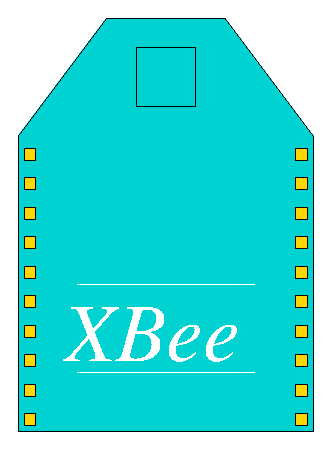
\includegraphics[width=0.4\linewidth]{figures/xbee.eps}
  \caption{XBee Series 2 with wire antenna
  \label{fig:xbee}}
\end{figure}

This device supports different kinds of ZigBee in mesh networking. Its wire antenna provides omnidirectional coverage, or what is the same as saying that its coverage is pretty much the same in all directions when the antenna is straight and perpendicular to the module.

If you flip the XBee, you will be able to see the pins through which it can send/receive data to/from sensors, communicate with Arduino, connection to a power supply and GND (more information about the pins can be found in page 15 of~\cite{faludi2010bws}).

\subsubsection{Preparing the XBee for configuration}

We can access and program the XBee through any terminal application and a USB connection. The \emph{breakout board} shown in Figure~\ref{fig:breakoutBoard} allows us to: $1$) plug the XBee into a breadboard, facilitating the wired connections with other components (including the Arduino); as well as the ability to $2$) establish a USB connection to configure the XBee.

\begin{figure}[htbp]
  \centering
  \includegraphics[width=0.4\linewidth]{figures/breakoutBoard.eps}
  \caption{XBee Explorer board from SparkFun
  \label{fig:breakoutBoard}}
\end{figure}

As the pins on the XBee are separated differently than the holes in the breadboard, every time a configuration or wired connection is needed, the XBee should be placed in the breakout board as shown in Figure~\ref{fig:xbeeAndBreakoutBoard}, and then placed on the breadboard.

\begin{figure}[htbp]
  \begin{center}$
    \begin{array}{cc}
      \includegraphics[width=0.4\linewidth]{figures/xbeeAndBreakoutBoard.eps}\label{xbeeOutside} &
      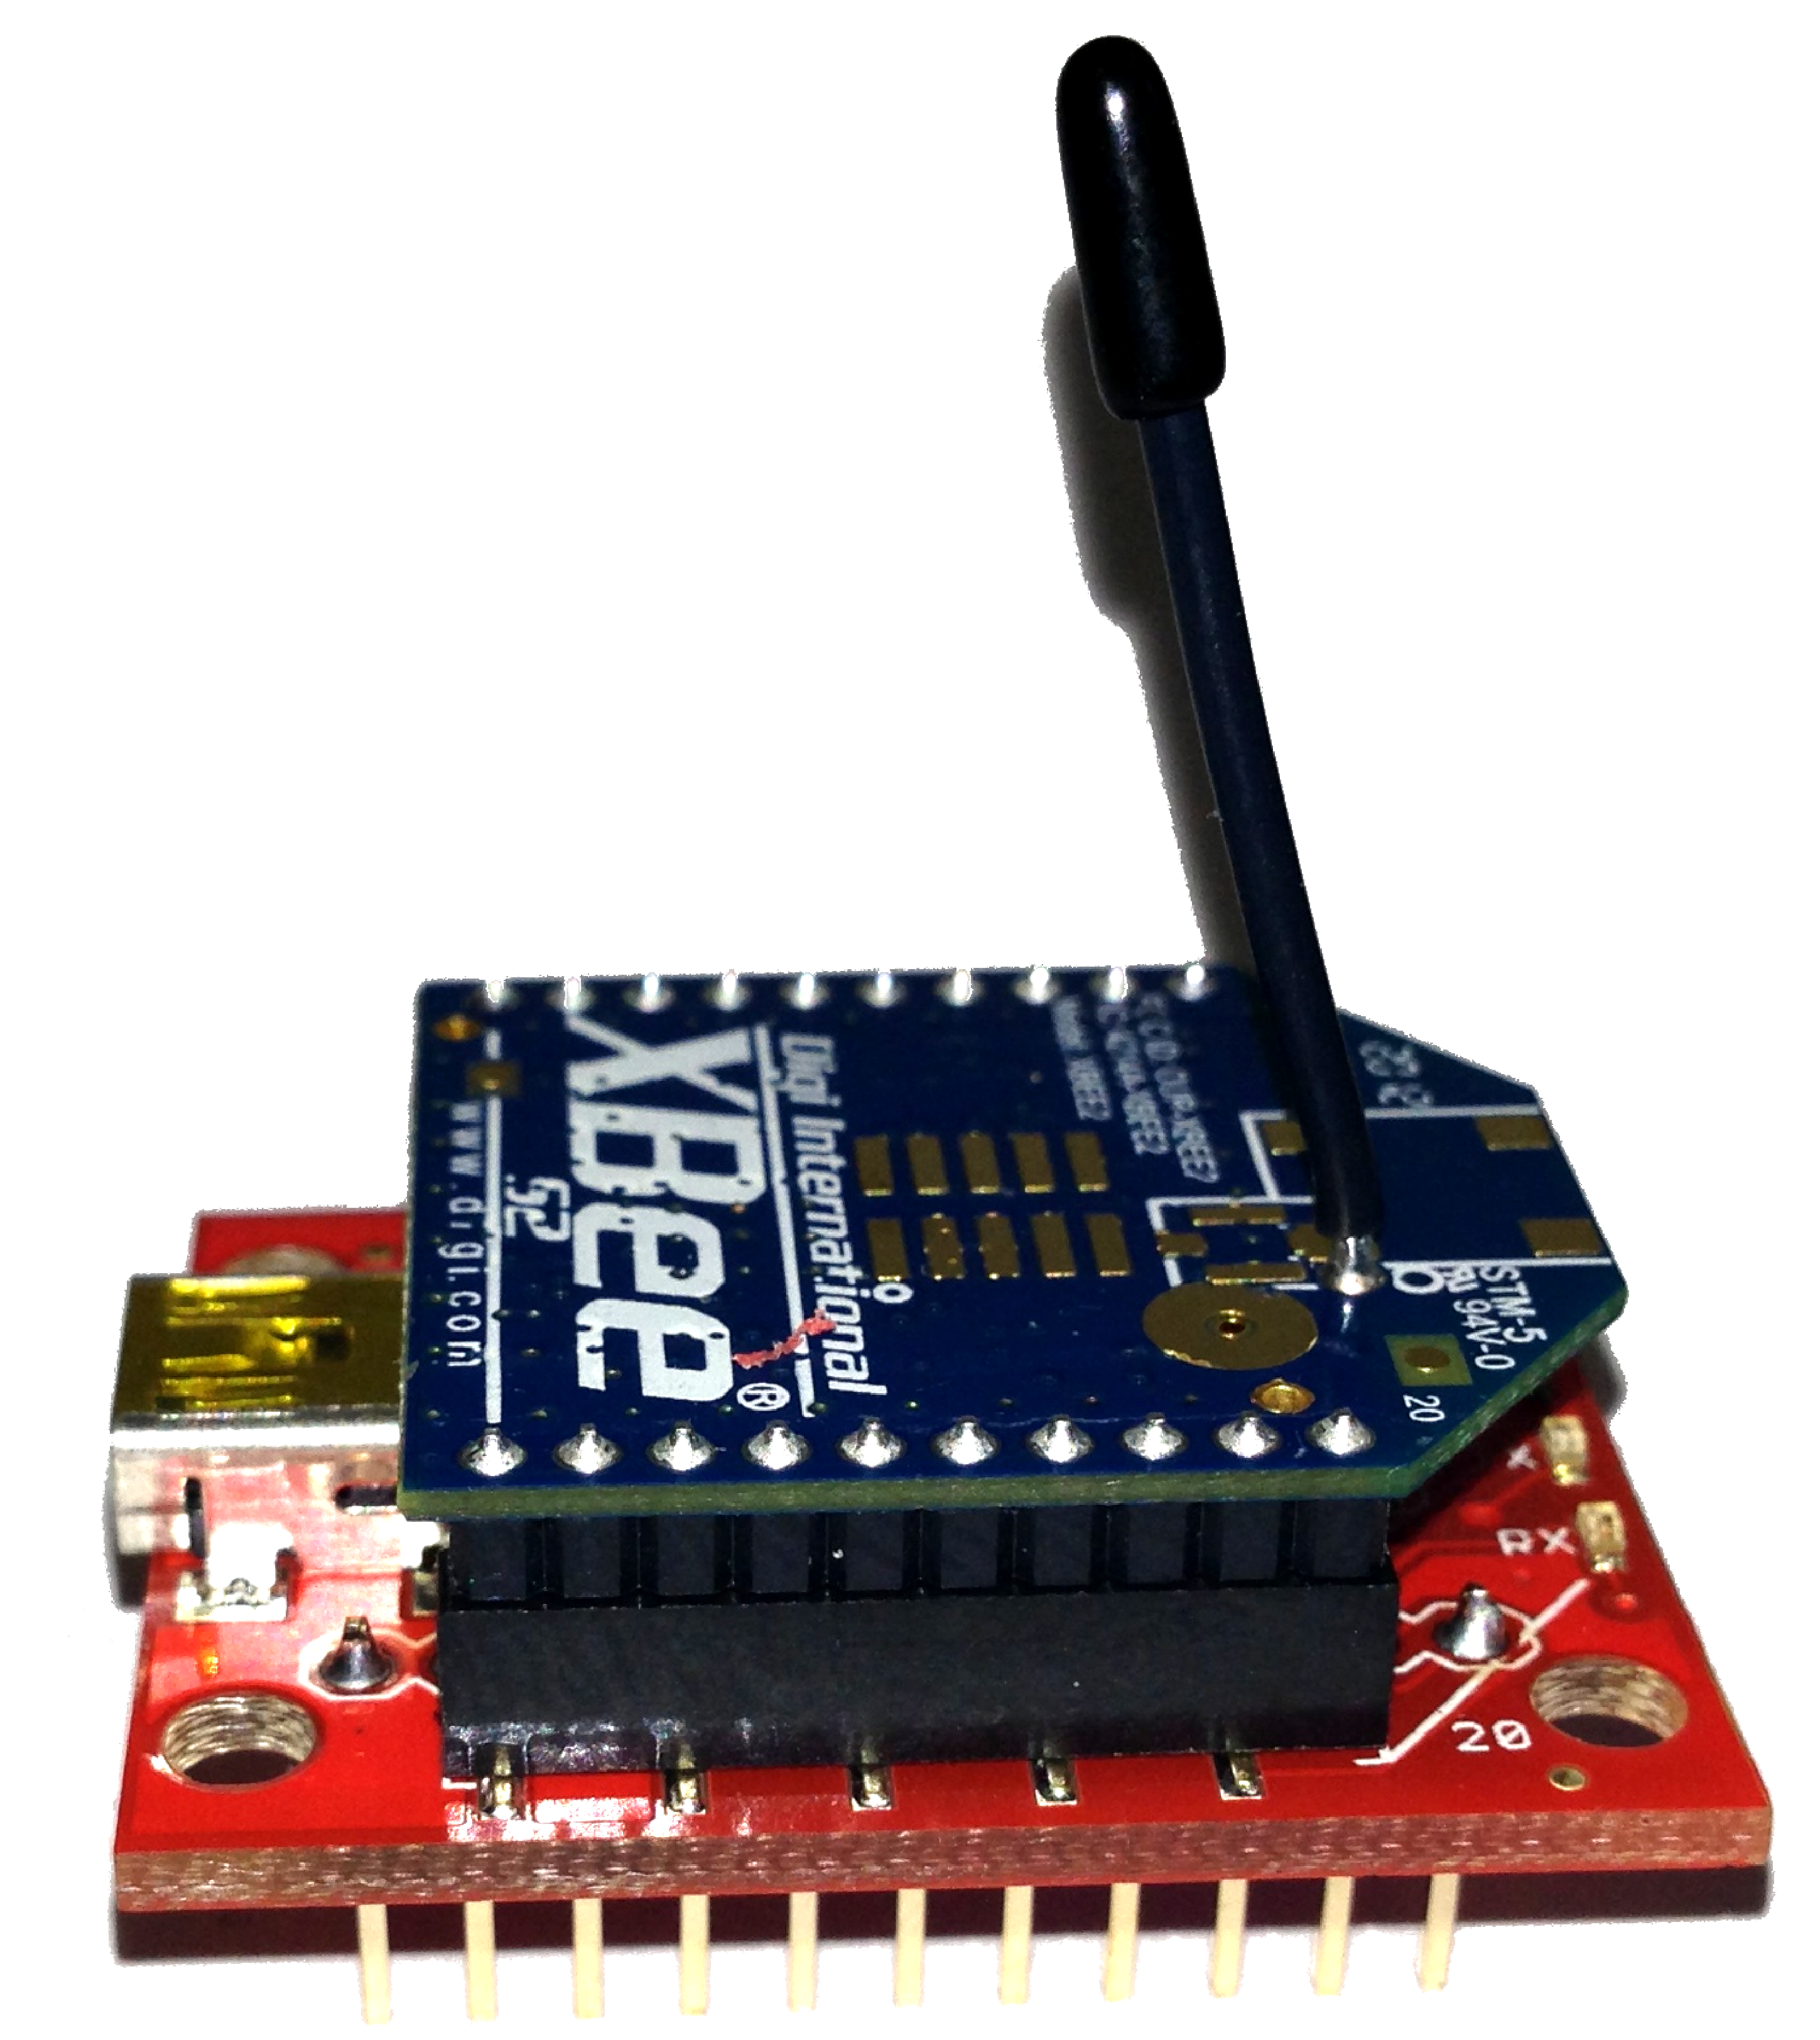
\includegraphics[width=0.4\linewidth]{figures/xbeeAndBreakoutBoard-inserted.eps}\label{xbeeInside}
    \end{array}$
  \end{center}
  \caption{XBee and breakout board: Left: XBee outside; see the different spacing of the pings. Right: XBee inside; setup for configuring and pluging into breadboard.
    \label{fig:xbeeAndBreakoutBoard}}
\end{figure}

It is important to notice that once the XBee is placed on the breakout board, the pins functions change. The new role of each pin is now the displayed underneath the breakout board, as in Figure~\ref{fig:xbeeBreakoutBoardPins}.

\begin{figure}[htbp]
  \centering
  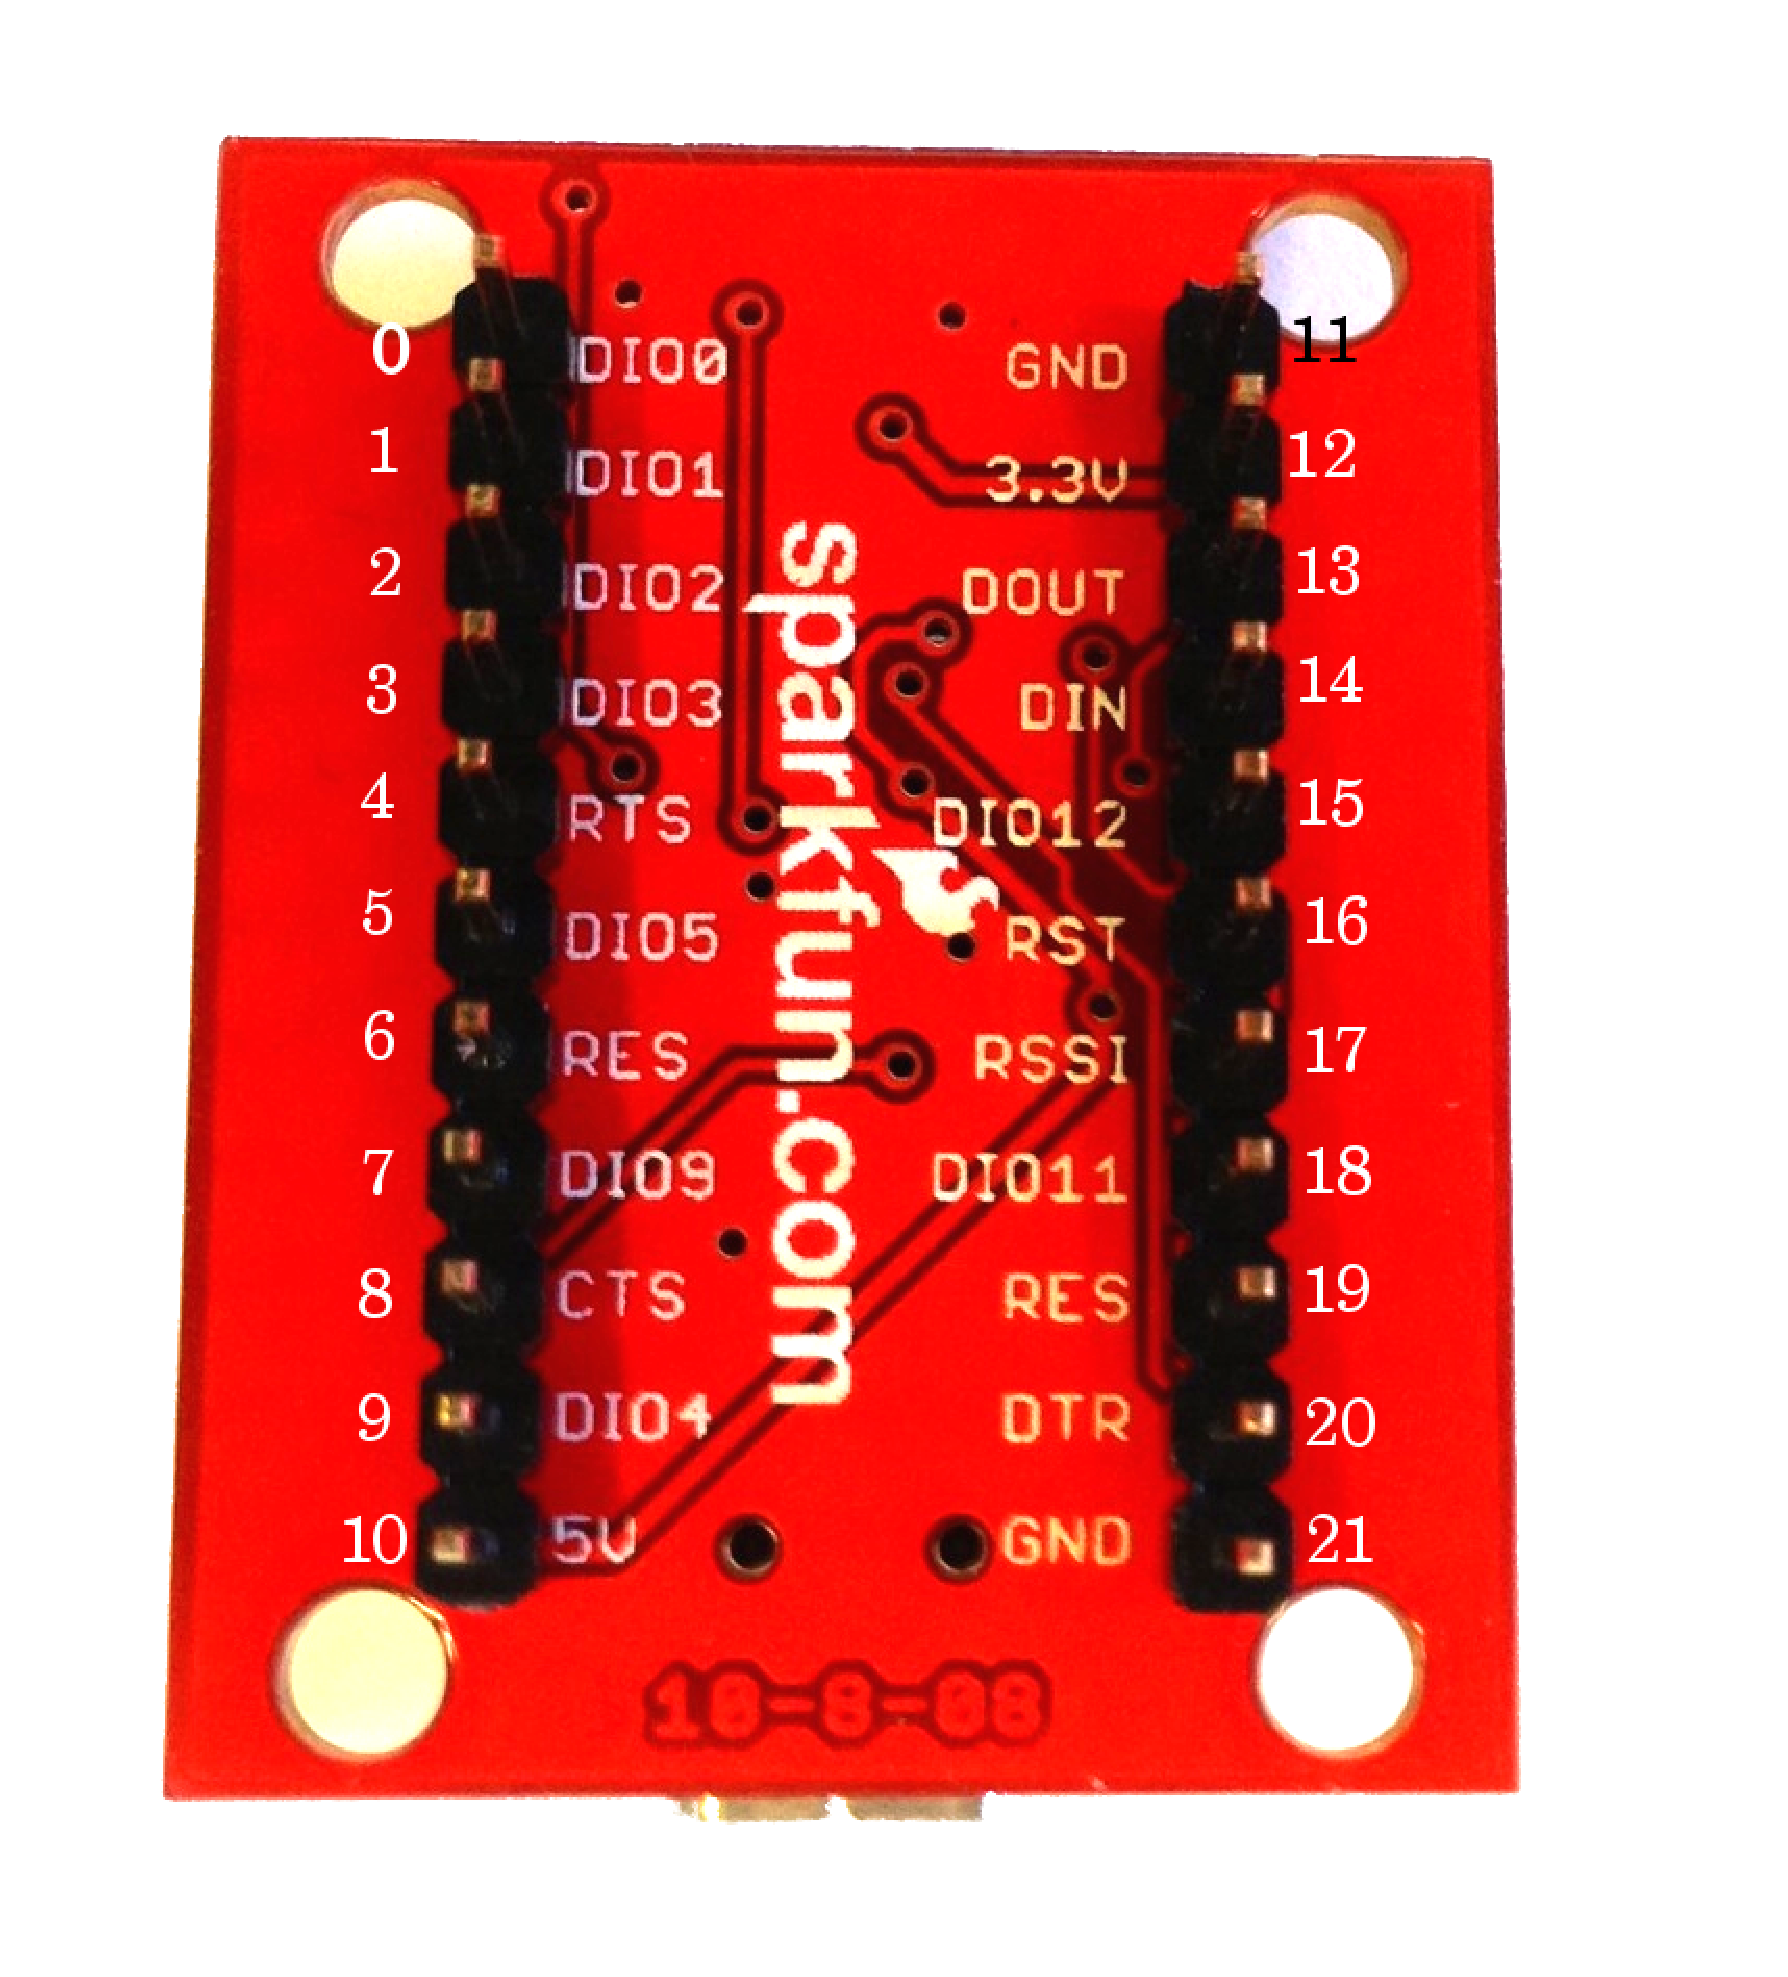
\includegraphics[width=0.6\linewidth]{figures/xbeeBreakoutBoardPins.eps}
  \caption{XBee Explorer pins
  \label{fig:xbeeBreakoutBoardPins}}
\end{figure}

Now that the device is properly placed, we need to setup a connection so the current configuration can be reviewed and changed.

\subsubsection{Accessing the firmware}\label{xbeeRoleConfiguration}

The XBee has a microcontroller running a configurable firmware. This firmware holds the necessary information for addressing, communication, security and utility functions. You can configure this firmware to change different settings like: local address, security settings, destination address and how the analog sensors connected to its pins are read.

As for now, the official way to update this firmware is through a program called \emph{X-CTU} and can be downloaded for free from the \emph{\color{blue}{\href{http://www.digi.com/support/kbase/kbaseresultdetl?id=2125}{XBee manufacturer's website}}}.

X-CTU is only available for the Microsoft Windows operating system, nevertheless you have the virtualization option in OS X, as well as WINE Windows emulator in Linux. 

To take a peek at the current XBee configuration: 

\begin{enumerate}
	\item Plug it into one of your computer's USB ports and launch the X-CTU application.
	\item Select the appropriate Com Port listed under \emph{Select Com Port}. This port should be the same in which your XBee is connected.
	\item Confirm that everything is setup correctly by clicking on the \emph{Test/Query} button. If everything is alright, a pop-up window will display the modem type and firmware version.
	\item Change to the \emph{Modem Configuration} tab on the top the X-CTU window. This tab will show you how the firmware is configured.
	\item Under \emph{Modem Parameters and Firmware}, click on the \emph{Read} button. This will fill the current window with the current firmware configuration, as well as the XBee's \emph{Modem} and \emph{Function Set}.
\end{enumerate}

Luckily, X-CTU is only required for upgrading the firmware. For changing the XBee's configuration we only need a USB connection and a terminal software. Nevertheless, this is only possible if the XBee is on \emph{AT command mode} (capable of receiving human commands and forward messages without performing any modification, see Table~\ref{tab:xbeeATModes}). To set it on, follow these steps:

\begin{enumerate}
	\item In the \emph{Model Configuration} tab of the X-CTU, check that the \emph{Modem type} is set to \texttt{XB24-ZB}.
	\item To start, we are going to configure two XBee radios. Under \emph{Function Set}, choose \texttt{ZIGBEE COORDINATOR AT}.
	\item Choose any version greater than \texttt{0x2070}.
	\item Click on the \emph{Write} button to program this device as a coordinator.
\end{enumerate}

Once the installation is complete, gently remove the USB from the first XBee radio a plug it into another. Repeat the process described above, but now under \emph{Function Set} choose \texttt{ZIGBEE ROUTER AT}. Select the highest version available and click on \emph{Write} to program the device.

It is important to distinguish between the two XBee you just configured, given that they behave differently. Every ZigBee network must contain only one coordinator radio, this way the network can be properly defined and managed. Mark which configuration each radio has with a sticker to eliminate any confusion.

\begin{table}[htbp]
	\centering
	\caption{XBee AT modes}
	\label{tab:xbeeATModes}
	\scalebox{0.7}{
	\begin{tabular}{c||c}
		\hline
		\bfseries Transparent mode & \bfseries Command mode\\
		\hline\hline
		Talk \emph{through} the XBee & Talk \emph{to} the XBee itself\\
		Any data can me sent through & Only responds to AT commands\\
		Default state & {\bfseries +++} to enter mode\\
		Wait $10$ seconds to return to this mode & Times out after 10 seconds of no input\\
		\hline
	\end{tabular}}
\end{table}

\subsubsection{Configuring the XBee through a terminal }

There are a lot of terminal applications. Fortunately, most of them need the same kind of information to establish a connection through USB. Table~\ref{tab:terminalParameters} gathers the required settings for a serial terminal software attempting to establish a connection with the XBee.

\begin{table}[htbp]
	\centering
	\caption{Default terminal settings for establishing a connection with an XBee}
	\label{tab:terminalParameters}
	\scalebox{0.7}{
	\begin{tabular}{c||c}
		\hline
		\bfseries Setting & \bfseries Value\\
		\hline\hline
		Baud & $9600$\\
		Data & $8$~bit\\
		Parity & None\\
		Stop bits & $1$\\
		Flow control & None\\
		Line feed & CR+LF or Auto Line Feed\\
		Local echo & on\\
		\hline
	\end{tabular}}
\end{table}

To check if you are already inside the XBee, try asking the radio to go to command mode issuing the \texttt{+++} instruction. If after a moment an \texttt{OK} appears at the right hand side, then you are in!

\subsubsection{Reviewing some AT commands for the XBee}

Issuing commands from a serial connection (like the one you established with the terminal program) to the XBee follows a simple guideline: \emph{instruction parameter} \texttt{<CR>}. Where \texttt{<CR>} accounts for \emph{carriage return}, and just means that you have to press the Return (Enter) key to submit the command. Passing and empty \emph{parameter} just outputs the current value of the specified register (the \emph{instruction} part of the command).

All AT commands start with the \texttt{AT} prefix (accounting for \emph{attention}) and then are followed by a two letter character command identification. Some of the basic AT commands are described below, as well as in~\cite{faludi2010bws}.

\begin{itemize}
	\item \texttt{AT}: gets the attention of the XBee. Its normal output is \texttt{OK}. If you do not receive this output,  you've probably timed out of command mode and need to reissue the \texttt{+++} command to get back in it.
	\item \texttt{ATID}: without any parameter it shows the current Personal Area Network ID (PAN ID) that is assigned to the radio. You can set a PAN ID passing an hexadecimal number in the range $0$x$0$-$0$xFFFF as a parameter.
	\item \texttt{ATSH/ATDL}: it shows the \emph{high} or \emph{low} parts of the unique XBee $64$-bit serial number, respectively. This number cannot be changed, so passing a parameter will produce an \texttt{ERROR} response.
	\item \texttt{ATDH/ATDL}: it shows the \emph{high} or \emph{low} parts of the \underline{destination} address the local radio will forward messages to, respectively. Putting address information after \texttt{ATDH} or \texttt{ATDL} will set the \emph{high} or \emph{low} parts of the destination address, accordingly.
	\item \texttt{ATWR}: saves the current configuration to firmware, so it will become the default configuration the next time you power on the XBee.
\end{itemize}

		

\chapter*{Lab Practices}\label{practices}

The following chapters gather all the labs hands-on practices that will guide through the process of setting schematics on your Arduino, configure a simple WSN, collect sensor data and upload it to a repository for future use.

Each practice suggests a chapter to read before attempting it. This way you will feel more familiarised with the terms used.

\emph{Code on!} \verb p(^-^q)


	\section{Practice: Installing the Arduino IDE}\label{pract:settingTheIDE}
In the following practice, you will spend some time getting to know the Arduino platform, its connections and how to interact with it through a PC.

\subsection{Reviewing the hardware}\label{pract:settingTheIDE:hardware}
As you were able to see in Figure~\ref{fig:Arduino_schematics}, the Arduino board contains a whole computer on a small chip, although it is at least a thousand times less powerful.

Taking a closer look at Figure~\ref{fig:Arduino_schematics}, you will be able to see \emph{14 Digital IO pins (pins 0-13), 6 Analogue IN pins (0-5) and 6 Analogue OUT pins (pins 3, 5, 6, 9, 10, and 11)}.

The \emph{Digital IO} pins, as the name suggests can be set to input or output. Their function is specified by the sketch you create in the IDE (more on IDE in Section~\ref{pract:settingTheIDE:IDE}). The \emph{Analogue IN} ports take analogue values (i.e., voltage readings from a sensor) and convert them into a number between 0 and 1023. As for the \emph{Analogue OUT} ports, are actually digital pins that can be reprogrammed for analogue output using the sketch you can create in the IDE.

\subsection{The Arduino IDE}\label{pract:settingTheIDE:IDE}
The Arduino Integrated Development Environment (IDE) is the responsible for making your code work in the Arduino board. Without entering in much unnecessary detail, what the IDE does is to translate your code into C language and compile it using \texttt{avr-gcc}, which makes it understandable to the micro-controller. This last step hides away as much as possible the complexities of programming micro-controllers, so you can spend more time thinking on your actual code.

You can download the Arduino IDE~\emph{\color{blue}{\href{http://www.arduino.cc/en/Main/Software}{from here}}}. If you are using \emph{Linux} or \emph{Windows} operating systems, just double click the downloaded file. This will open a folder named \emph{arduino-[version]}, such as \emph{arduino-1.0}. Place the folder wherever you want in your system. On the Mac, just double click the downloaded file, this will open a disk image containing the Arduino application. Drag a drop the application icon to your Applications folder.

Do not open your installed application yet. First you must teach your computer to detect the Arduino hardware through the USB ports.

\subsubsection{Configuring the USB ports for detecting the Arduino}
In Linux and OS X, the USB controllers are the same used by the operating system.

\emph{\bf{On the Mac}}, plug the Arduino into an USB port.

The PWR light on the board should come on. Also, the LED labelled "L" should start blinking.

Then, a pop-up window telling you that a new network interface was found should appear. Proceed clicking "Network Preferences...", and then "Apply". Although it may appear with a status of "Not Configured", the Arduino is ready for work.

\emph{\bf{Windows}} machines, plug your Arduino and the ``Found new Hardware Wizard'' will appear. After the wizard tries to find the driver on the Internet, you will be able to select "Install from a list or specific location" button. Choose it and click next. You will be able to find the drivers under the "Drivers" folder of the Arduino Software download.

Once the drivers are installed, you can launch the IDE and start using Arduino.

\subsubsection{Identifying the port connected to the Arduino}
In the case of the \emph{\bf{Mac}}, once in the Arduino IDE, select "Serial Port" from the "Tools" menu. Select \texttt{/dev/cu/.usbmodem}; this is the name that your computer uses to refer to the Arduino board.

For \emph{\bf{Windows}}, under the operating system "Start" menu open the "Device Manager" by right-clicking on "Computer" (Vista) or "My Computer" (XP), then choose properties. On XP, click "Hardware" and choose Device Manager. On Vista, click "Device Manager".

Look for the Arduino device in the list under "Ports (COM \& LPT)". Your device name will be followed by a port number, usually "COM\#", where \# refers to a number.

Once you have identified the COM port number for the Arduino connection, you can select that port from the Tools~$>$~Serial Port menu in the Arduino IDE.

Now the Arduino IDE can talk with the Arduino board and program it.

\subsubsection{What's the deal with Linux users?}
As mentioned before, IDE uses the same USB controllers than Linux. So, in order to effectively detect your Arduino in Linux, simply connect it to your PC, open a Terminal a type \texttt{ls dev/ttyUSB*}. This will display all available ports. Your Arduino serial port will probable be something like \texttt{/dev/ttyUSB0}.

	\section{Practice: Blinking LED}\label{pract:blinkingLED}
In the following practice you will write your first Arduino application. Although simple, mastering it will provide you with clear understanding of the IDE and the components that conform the Arduino platform.

It consist of a simple code that will turn on/off LED(s) plugged to the digital IO ports of the Arduino.

\subsection{Preparing your development environment}
For Practice~\ref{pract:blinkingLED}, you will need:
\begin{itemize}
 \item as many LEDs as you want, but always less than the number of digital IO ports.
 \item a USB cable to connect your Arduino board to the PC.
 \item the Arduino IDE, up and running.
\end{itemize}

Turn on your Arduino by plugging it to the PC. Make sure you have selected the appropriate COM port, as it is explained in Practice~\ref{practice1-1} according with your operating system.

\subsection{The code}
Once inside, enter the following code:

\begin{verbatim}
const int LED = 13; // LED connected to 
                    //digital pin 13
void setup()
{
  pinMode(LED,OUTPUT); // sets the digital
                       // pin as output
}
void loop()
{
  digitalWrite(LED, HIGH); //turns LED on
  delay(1000);             //waits 1000ms
  digitalWrite(LED, LOW);  //turns LED off
  delay(1000);
}
\end{verbatim}

As you might be able to see, the code is completely readable. Let's review it line by line.

\begin{itemize}
 \item \texttt{const int LED = 13}: assigns the value $13$ to a \texttt{\color{red}{int}}erger variable, named LED. In this case, this number corresponds to the digital IO port \#13.
 \item \texttt{void setup()} is the name of the next block of code. It is very similar to functions in languages like C/C++.
\end{itemize}

	\section{Practice: Blinking LED Advanced}\label{pract:blinkingLEDAdvanced}

It will be very boring to just have a blinking LED. That is because in this practice we will be incorporating some hardware and software tweaks that will allow us to have a little more control over the LED. Or let's say, we will make a basic lamp.

What we want to prototype is a LED that turns on or off whenever we press a bottom. Before we dwell into detail, let's review what we will need:

\begin{itemize}
	\item A breadboard (we will be using Figure~\ref{fig:breadboard} as a guide).
	\item Wire to tie together the different parts of your circuit.
	\item One $10$K Ohm resistor.
	\item One pushbutton switch.	
\end{itemize}

\begin{figure}[htbp]
  \centering
  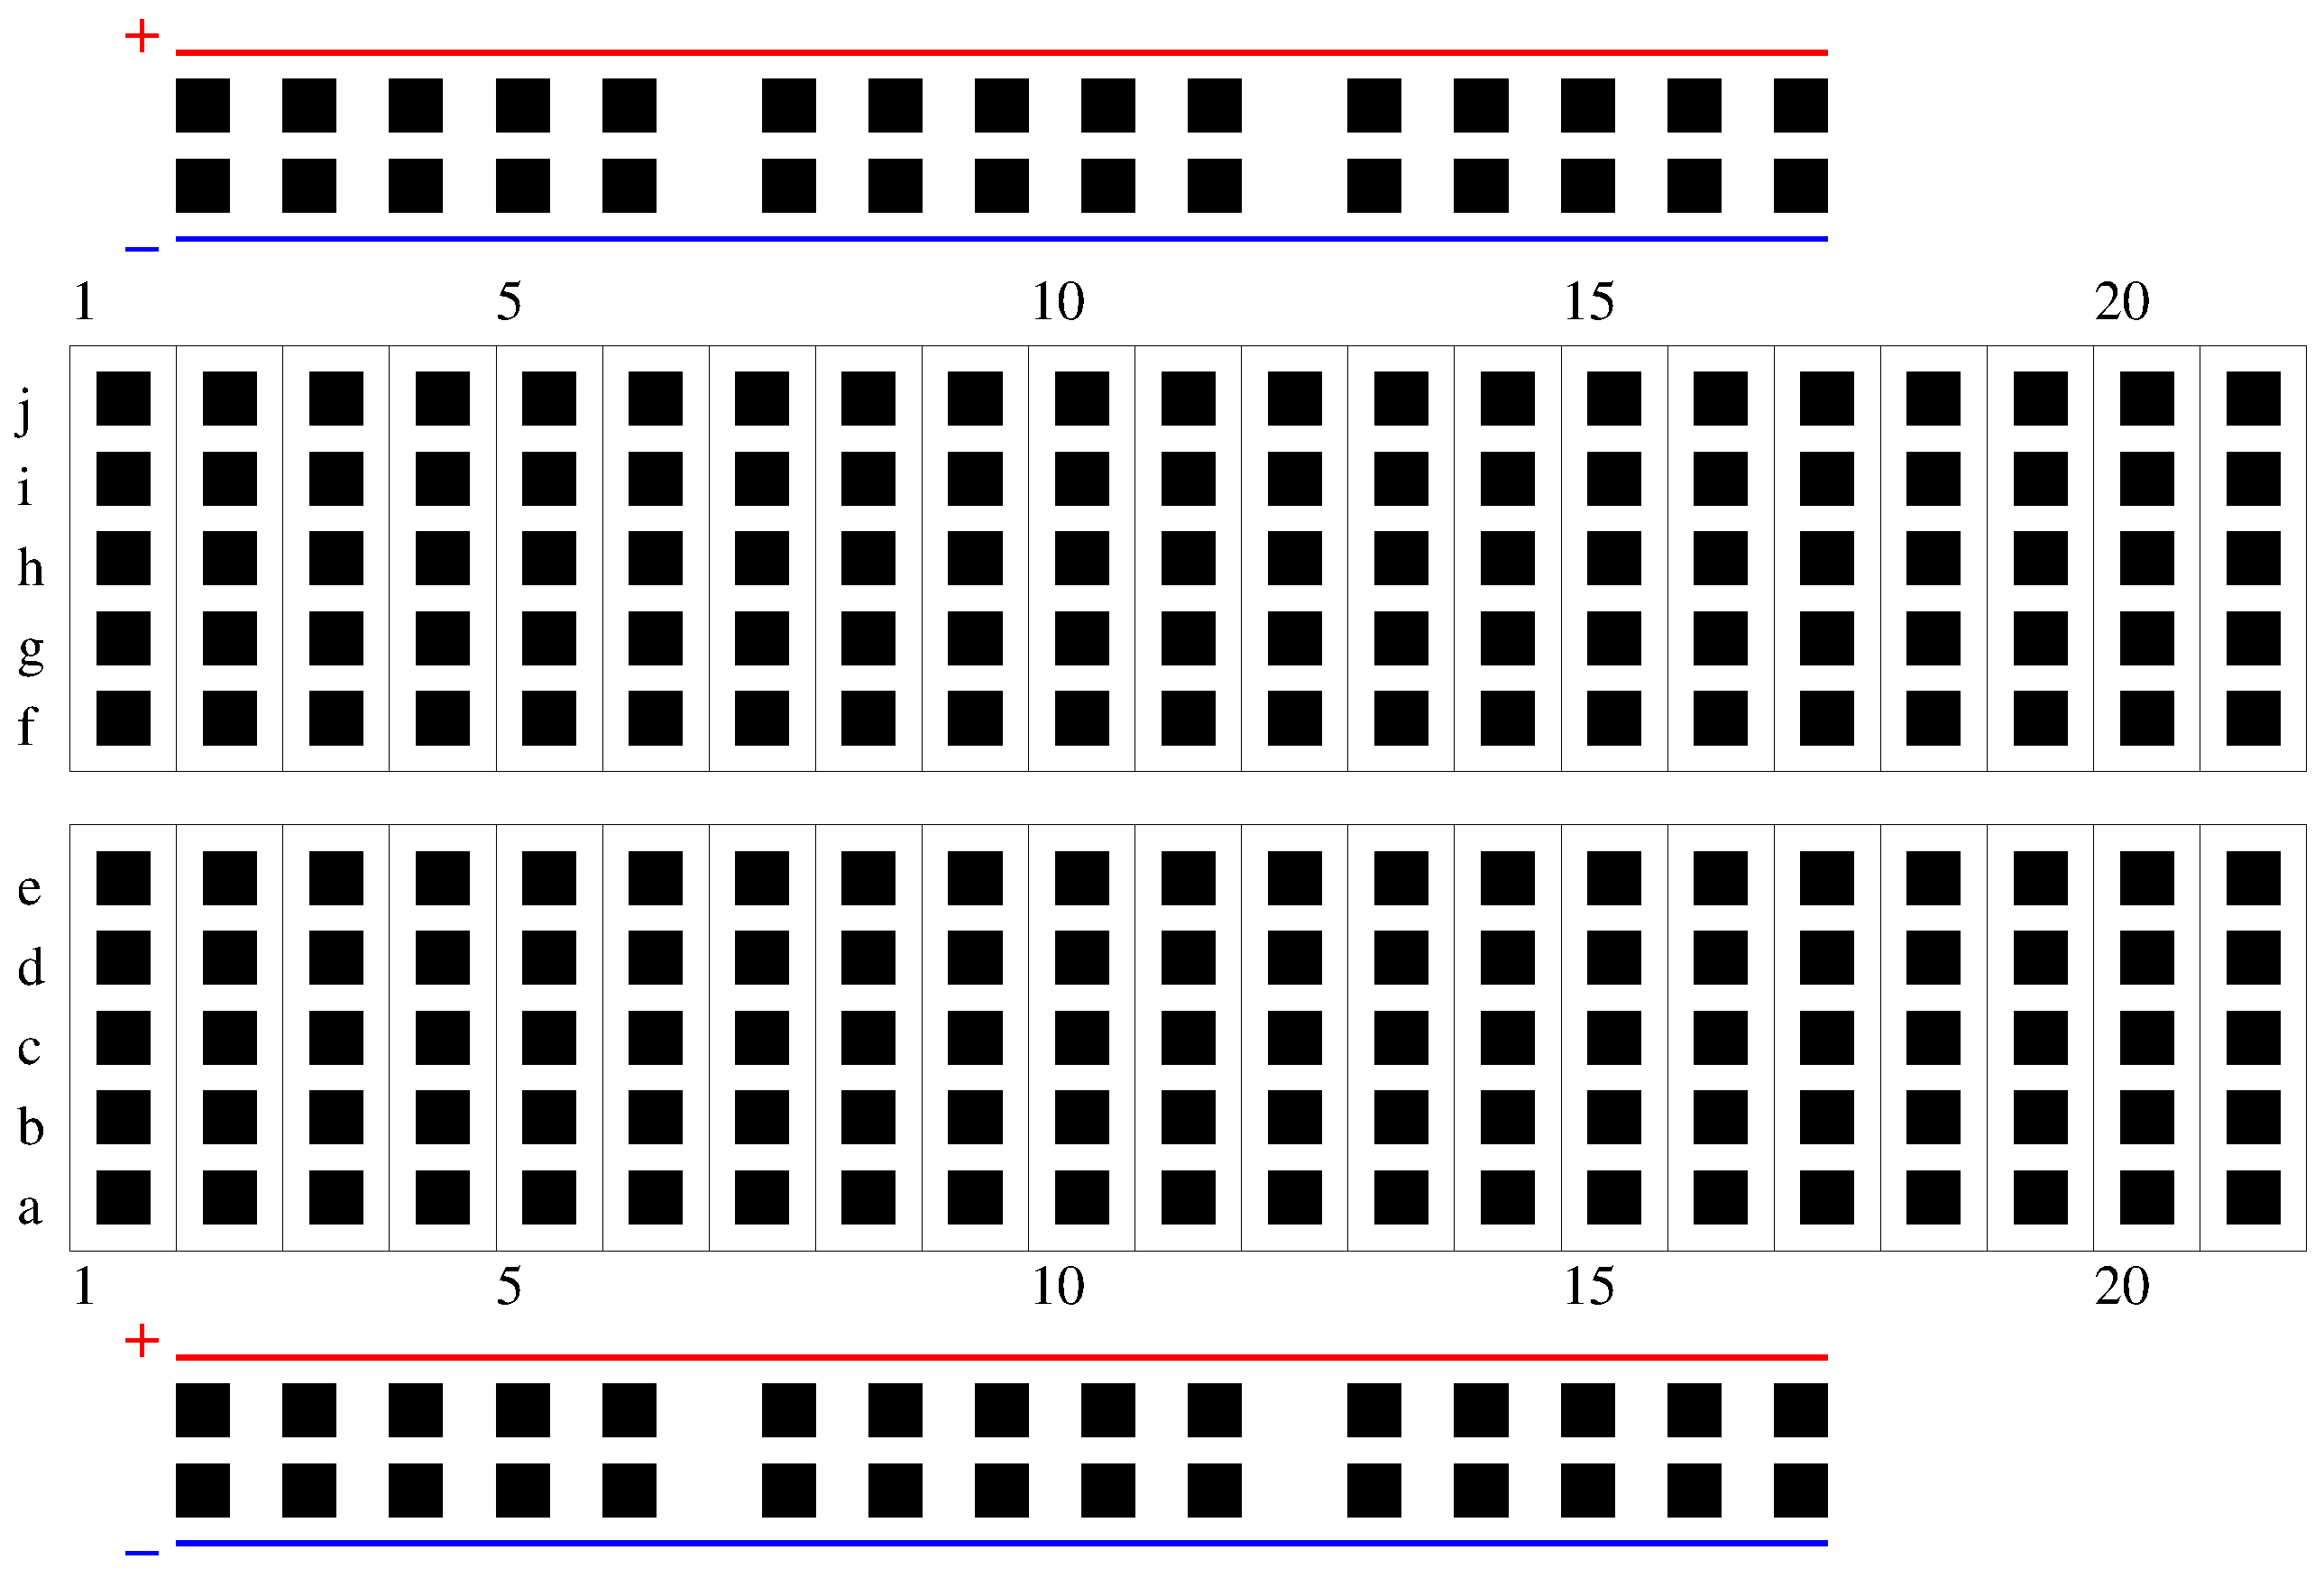
\includegraphics[width=0.7\linewidth]{figures/breadboard.eps}
  \caption{Breadboard
  \label{fig:breadboard}}
\end{figure}

Breadboards will help us to build circuits. It allows for effective connection between components without worrying about the electrical subtleties or hazards. Taking Figure~\ref{fig:breadboard} as a reference, the breadboard has internal electrical connections that makes it possible to tie multiple components to a single point. It does so by representing a \emph{physical} connection as multiple rows of the same column. That is: holes $1$a and $1$d are physically connected inside the breadboard's circuitry, whereas $3$d and $4$a are not.

Each breadboard is divided by thick spaces among different sections. In Figure~\ref{fig:breadboard}, there are four distinct sections: two with the $+$ and $-$ symbols, and two with numbers and letters. The latter was described above, whereas the former works in the opposite way: holes are connected with other holes in the same row. This section is often used to power the circuit, but more on that further in the practice.

Before writing any code, try to assemble the parts as shown in Figure~\ref{fig:blinkingLEDAdvancedLayout}.

\begin{figure}[htbp]
  \centering
  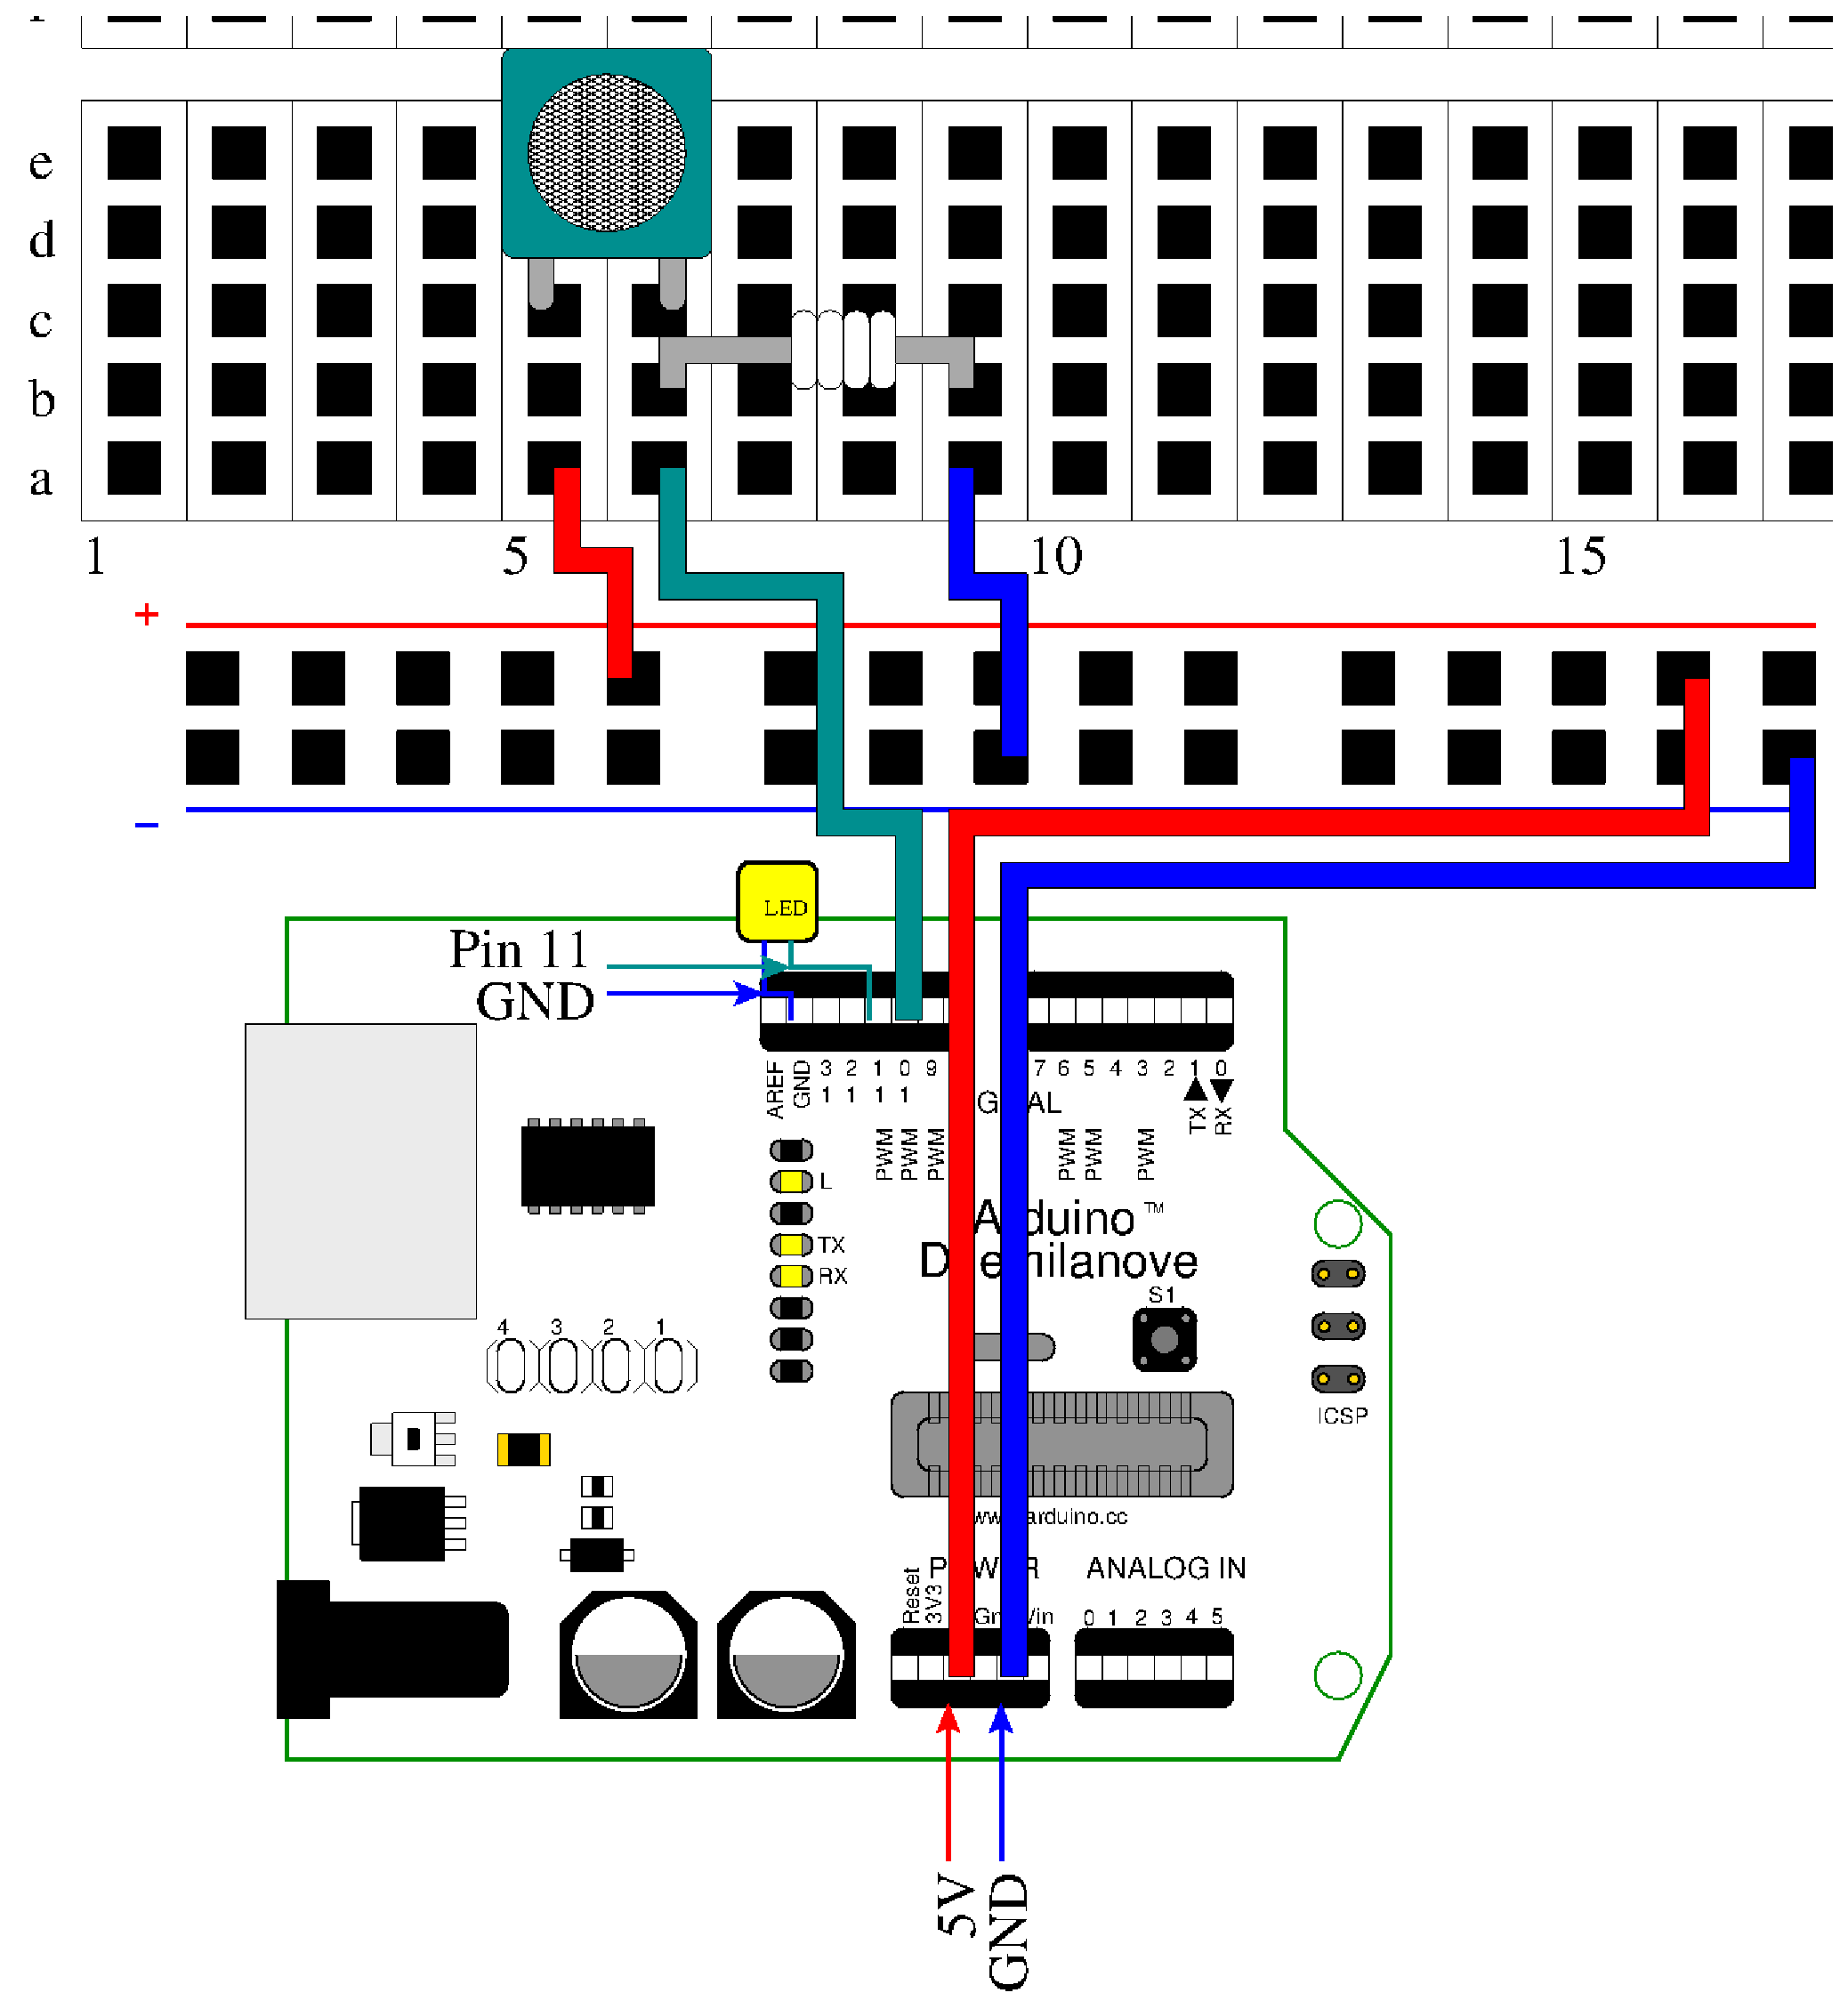
\includegraphics[width=0.7\linewidth]{figures/blinkingLEDAdvanced-scaled.eps}
  \caption{Blinking LED advanced layout
  \label{fig:blinkingLEDAdvancedLayout}}
\end{figure}

To avoid any confusion, let's review the layout component by component:

\begin{enumerate}
	\item Place the pushbutton on your breadboard. In Figure~\ref{fig:blinkingLEDAdvancedLayout}, the two pushbutton "legs" are inserted into holes $5$c and $6$c. In this example, the pushbutton will be energised through the $5$c leg.
	\item Connect one of the legs of the resistor to the negative leg of the pushbutton (hole $6$b). This will physically connect the resistor to one of the legs of the pushbutton. Insert the other leg on hole $9$b.
	\item In order to avoid confusion, cables on all figures are color coded. \emph{Red} represents power cables, \emph{blue} are connections to GND and \emph{cyan} are connections to IO pins on the Arduino.
\end{enumerate}
	\chapter{Practice: Simple chat with XBee}\label{pract:simpleChat}
\section*{Suggested read: Chapter \ref{introToXBee}}

WSNs are composed of nodes able to send messages among themselves. In this practice you will be guided through the configuration of (at least) two XBees to build a basic chat application. Furthermore, you will have the opportunity to familiarize yourself with the XBee and the different AT commands described in Chapter~\ref{introToXBee}.

You will need:

\begin{itemize}
	\item One XBee Series 2 configured as a \texttt{ZIGBEE COORDINATOR AT}.
	\item One XBee Series 2 configured as a \texttt{ZIGBEE ROUTER AT}.
	\item As many breakout boards and USB cable A to mini B as XBee radios.
	\item One computer per XBee. It is less confusing than establishing multiple terminal sessions from one computer.
\end{itemize}

We need to be able to distinguish the coordinator radio from the router radios. It is easier if you write this addresses down. Proceed as follows:

\begin{enumerate}
	\item Establish a terminal connection to the coordinator radio.
	\item Once inside, issue the \texttt{+++} to enter to command mode.
	\item Type \texttt{ATSL} to reveal the lower part of the XBee serial number.
	\item Write it down: {\bfseries Coordinator address:} $0013$A$200$ \underline{\ \ \ \ \ \ \ \ \ \ \ \ }
\end{enumerate}

Repeat the same for the router AT.

{\bfseries Router address:} $0013$A$200$ \underline{\ \ \ \ \ \ \ \ \ \ \ \ }

Now, let's configure the coordinator.

\section{The code: coordinator}

The settings for the coordinator are contained in Table~\ref{tab:xbeeChatCoordinator} below.

\begin{table}[htbp]
	\centering
	\caption{XBee coordinator settings for simple chat}
	\label{tab:xbeeChatCoordinator}
	\scalebox{0.7}{
	\begin{tabular}{c||c||c}
		\hline
		\bfseries Description & \bfseries Command & \bfseries Parameter\\
		\hline\hline
		PAN ID & \texttt{ATID} & {\bfseries 2013}\\
		Destination address \emph{high} & \texttt{ATDH} & {\bfseries 0013A200}\\
		Destination address \emph{low} & \texttt{ATDL} & {\bfseries\underline{\ \ \ \ \ \ \ \ \ \ \ \ }}\\
		\hline
	\end{tabular}}
\end{table}

Note that the \emph{Destination address low} specified in Table~\ref{tab:xbeeChatCoordinator} correspond to the \underline{router} radio.

Issuing the commands on the terminal window will look like the listing below.

\begin{lstlisting} [caption = {Coordinator settings as seen in the terminal}, label = {code:xbeeChatCoordinator}, numbers = left, escapeinside={@}{@}]
+++
OK
ATID 2013
OK@\label{SC:instructionOK}@
ATDH 0013A200
OK
ATDL ____ //put the lower part of the router address
OK
ATID
2013
ATDH
0013A200
ATDL
____
ATWR
OK@\label{SC:writeOK}@
\end{lstlisting}

You will receive an \texttt{OK} after issuing a command (as in Line~\ref{SC:instructionOK}) as well as when writing to the firmware (Line~\ref{SC:writeOK}).

\section{The code: router}

The settings for the router must contain the same information collected for the coordinator. Fill out Table~\ref{tab:xbeeChatRouter} accordingly.

\begin{table}[htbp]
	\centering
	\caption{XBee router settings for simple chat}
	\label{tab:xbeeChatRouter}
	\scalebox{0.7}{
	\begin{tabular}{c||c||c}
		\hline
		\bfseries Description & \bfseries Command & \bfseries Parameter\\
		\hline\hline
		PAN ID & \texttt{ATID} & {\bfseries 2013}\\
		Destination address \emph{high} & \texttt{ATDH} & {\bfseries 0013A200}\\
		Destination address \emph{low} & \texttt{ATDL} & {\bfseries\underline{\ \ \ \ \ \ \ \ \ \ \ \ }}\\
		\hline
	\end{tabular}}
\end{table}

Note that the \emph{Destination address low} specified in Table~\ref{tab:xbeeChatRouter} correspond to the \underline{coordinator} radio.

\subsection{Chat!}
Now you just have to connect each XBee to one computer and establish a terminal connection to each one (or connect the two radios to the same computer running two different terminal applications, one for each XBee). Make sure all the connection settings are as specified in Table~\ref{tab:terminalParameters}, so you will not have any problems.

If both radios are in transparent mode (see Table~\ref{tab:xbeeATModes}), everything you type in one terminal will be forwarded to the other XBee.

\section{Next Steps}

Other things you can try:

\begin{itemize}
\item Create a chat involving the whole class in a single network.
This should be a broadcast chat in which everyone receives all the messages.
\item Now, using a single large network, use the destination address to chat between two XBees.
Do not include the 16 bits address.
\item  Try again including the 16 bits address
\item  Try again flashing at least one node as an end device.
\end{itemize}

	\chapter{Practice: Wireless doorbell}\label{pract:wirelessDoorbell}
\section*{Suggested read: Chapters~\ref{introToXBee} and~\ref{pract:simpleChat}}

This practice guides you through the construction of a wireless doorbell system. It is composed by two components: the switch and the buzzer.

On the switch side, we will be prototyping a layout like the one shown in Figure~\ref{fig:wirelessDoorbellSwitch}. While the sound will be produced by a buzzer on the other radio, like in Figure~\ref{fig:wirelessDoorbellBuzzer}.

You will need:

\begin{itemize}
  \item Eventhough the two components may fit in one breadboard; to make it more real, it is better to use two separate breadboards.
  \item Hookup wire. It is recommended to have at least four different colors.
  \item Two Arduino boards.
  \item USB A-to-B cable for the Arduinos.
  \item One $10$K$\Omega$~resistor.
  \item One momentary switch or pushbutton for input.
  \item One buzzer for output.
  \item One XBee radio configured as \texttt{ZIGBEE COORDINATOR AT}.
  \item One XBee radio configured as \texttt{ZIGBEE ROUTER AT}.
  \item Two breakout boards.
  \item USB cable for the XBee breakout board.
\end{itemize}

Every ZigBee network has only one coordinator. Other nodes can be configured as routers. To configure your XBee radios, please refer to Chapter~\ref{xbeeRoleConfiguration}.

It is strongly suggested that you mark down the XBees to distinguish the coordinator from the router(s).

\section{Wireless doorbell connections layout}

\subsection{Switch}
Follow these guidelines to prepare the connections for the switch that will make the doorbell ring (or buzz in our case). If lost, you can always take a look at the final layout in Figure~\ref{fig:wirelessDoorbellSwitch}.

\begin{enumerate}
  \item Energize the breadboard by hooking up a {\color{red}{red}} wire from the Arduino $3.3$V output to one of the power rails of the breadboard.
  \item Hook up a {\color{blue}{blue}} wire from the ground (GND) connection on the Arduino to the ground rail on the breadboard.
  \item Place the XBee/breakout board with both sides on different sections of the breadboard, in a way that the space separating the sections passes under the XBee/breakout board.
  \item Use a {\color{red}{red}} wire to connect pin $3.3$V (or pin $1$ as in Figure~\ref{fig:xbeeBreakoutBoardPins}) of the XBee to the power rail on the breadboard.
  \item Use another color cable to hookup the XBee's GND pin to the ground in the breadboard.
  \item Grab another color cable to connect pin TX/DOUT of the XBee to digital pin 0 (RX) on the Arduino.
  \item Then do the reverse way communication by connecting XBee's RX/DIN pin to the digital pin 1 (TX) on your Arduino.
  \item With the coordinator XBee, attach the button to the digital input 2 of your Arduino, making sure to use the 10K$\Omega$ resistor as in Figure~\ref{fig:wirelessDoorbellSwitch}.
\end{enumerate}

The other XBee (as a router) will work as the buzzer. For this, replicate the schematics shown in Figure~\ref{fig:wirelessDoorbellBuzzer}.

\begin{figure}[htbp]
  \centering
  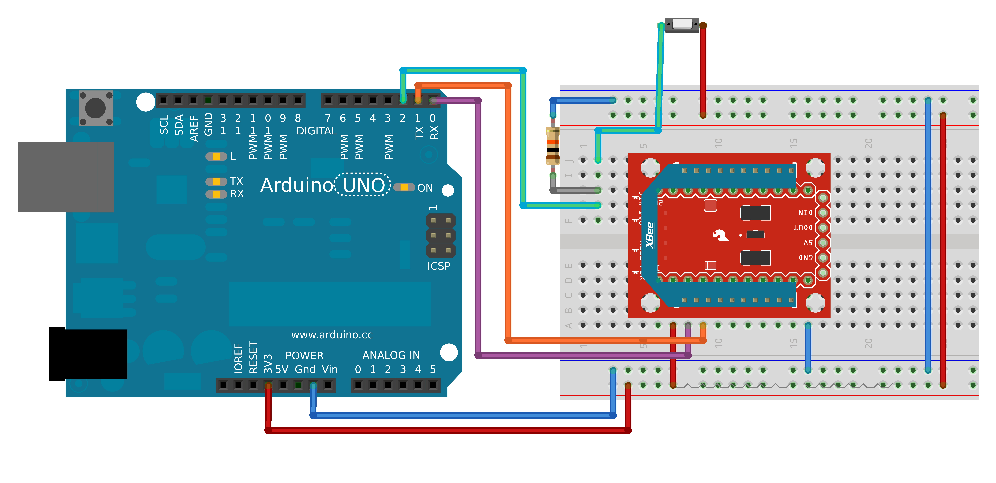
\includegraphics[width=\linewidth]{figures/doorbellSwitch-NEW.eps}
  \caption{Wireless doorbell: switch layout
  \label{fig:wirelessDoorbellSwitch}}
\end{figure}

\begin{figure}[htbp]
  \centering
  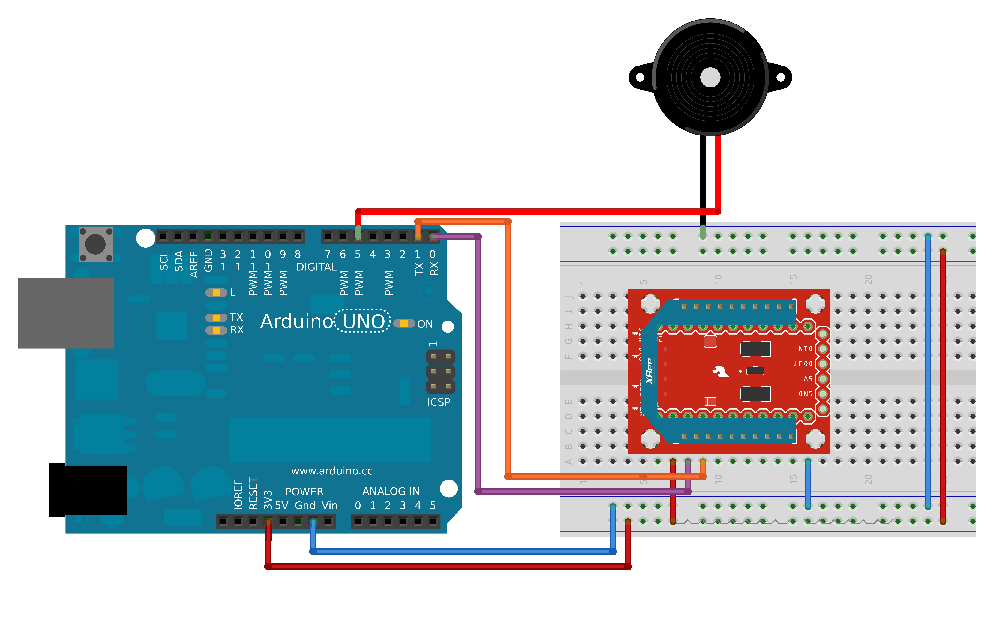
\includegraphics[width=\linewidth]{figures/doorbellBuzzer-NEW.eps}
  \caption{Wireless doorbell: buzzer layout
  \label{fig:wirelessDoorbellBuzzer}}
\end{figure}

\section{The code}\label{wirelessDoorbellCode}
\subsection{XBee code}

First, start with the coordinator. It is recommended that you attach a sticker or some kind of mark to each XBee so you will know which one is the coordinator and the router.
\begin{enumerate}
  \item Start a terminal session with the XBee. You can use any terminal application or the terminal utility in the X-CTU.
  \item To start interactive mode, type \texttt{+++} and the XBee will respond with an \texttt{OK} message. You're in!
  \item Select a PAN ID number between 0x0 and 0x(16 Fs), so there are plenty PAN IDs. Then, configure the XBee to work in this PAN ID by entering \texttt{ATID} followed by the PAN ID you selected and press enter. The XBee should respond with an \texttt{OK} message. If not, then maybe you were thrown out of command mode. Retry by issuing the \texttt{+++} command again.
  \item Because we are working with a pair of radios, this one should have as a destination address the address of the other XBee you are using. So, enter the \emph{high} part of the other XBee destination address by typing \texttt{ATDH 0013A200}.
  \item Then, enter the \emph{low} part of the destination address by typing \texttt{ATDL} followed by your other XBee's lower address.
  \item Write your configuration by issuing \texttt{ATWR} and pressing enter.
\end{enumerate}

Repeat this same process with your other XBee. Remember that:

\begin{itemize}
  \item You will be thrown out of command mode after 10 seconds of inactivity. To re-enter enter the \texttt{+++} command and wait for the \texttt{OK} response.
  \item The destination addresses are those of the other XBee! This is a frequent mistake.
  \item After making changes, always save them by entering the \texttt{ATWR} command.
\end{itemize}

\subsection{The Arduino code}
\subsubsection{The button Arduino}
This code corresponds with the button side of the example.
\\
{\color{red}{There's a trap!}}: when uploading programs to your Arduino, disconnect the digital pin 0 (RX) and then reconnect it after the loading is completed. Otherwise you will receive an error.

\begin{lstlisting} [caption = {Configuring the Arduino of the buttom side of the example.}, language = C, label = {code:wirelessDoorbellButton}, numbers = left, escapeinside={@}{@}] 
int BUTTON = 2;
void setup() { 
	pinMode(BUTTON, INPUT); 
	Serial.begin(9600);
}
void loop() {
// send a capital D over the serial port if the button is pressed
	if (digitalRead(BUTTON) == HIGH) { 
		Serial.print('D');
		delay(10); // prevents overwhelming the serial port 
	}
}
\end{lstlisting}

\subsubsection{The buzzer Arduino}
This Arduino will receive a signal when the button is pressed and will ring the buzzer.

\begin{lstlisting} [caption = {Configuring the Arduino of the buzzer side of the example.}, language = C, label = {code:wirelessDoorbellBuzzer}, numbers = left, escapeinside={@}{@}]
int BELL = 5;
void setup() { 
	pinMode(BELL, OUTPUT); 
	Serial.begin(9600);
}
void loop() {
	// look for a capital D over the serial port and ring the bell if found 
	if (Serial.available() > 0) {
		if (Serial.read() == 'D'){ 
		//ring the bell briefly 
			digitalWrite(BELL, HIGH); 
			delay(10); 
			digitalWrite(BELL, LOW);
		}		 
	}
}
\end{lstlisting}

\section{Next Steps}
\begin{itemize}
\item The Arduino on the buzzer side can send a confirmation to the Arduino on the push-button side.
This confirmation means that the initial message has been received and the buzzer is buzzing.
Include an additional LED on the switch side that lights up when this confirmation is received.
Now try the doorbell again.
Confirm that the LED lights up when the button is pushed.
Finally, disconnect the Arduino on the buzzer side and try to push the button again.
There should be no sound and no light.
\item Make a more sophisticated doorbell.
Include an LED on the buzzer side.
When the button is pressed, the LED lights up.
When the button is pressed for longer than one second, the buzzer buzzes.
\item The challenge. The buzzer side has a light sensor. During the day, it behaves as a regular buzzer.
If it is dark, it lights up a LED and sounds the buzzer only when the button has been pressed for over three seconds.
The buzzer side sends feedback to the button side.
The button side will blink a LED while the remote LED is on and turn on a steady LED when the buzzer is being sounded.

\end{itemize}






    \chapter{Practice: A WSN with XBee's AT mode}\label{ATSensorNetwork}
\section*{Suggested read: Chapers~\ref{introToXBee},~\ref{pract:simpleChat} and~\ref{pract:thermometer}}

In this assignment we will build a sensor network using the AT (as opposed to the API) mode.
This means that we will directly write characters in one end and read them at the other end.
We can replace any of the two ends by a serial terminal emulation (\emph{\color{blue}{\href{http://en.wikipedia.org/wiki/Minicom}{minicom}}}).

We start by flashing two XBees using X-CTU.
We will install the AT firmware in them.
One has to be the coordinator and the other the router.

Then we have to configure the PANID, and the destination address for each of them.
The configuration can be done using X-CTU or the minicom.
Verify the configuration observing the RSSI LED and then connecting minicom to both XBee and sending information from one XBee to the other as in the chat assignment (see Chapter~\ref{pract:simpleChat}).

We will use one of the XBees on the solderless breadboard, connected to the Arduino.
As usual, use the Arduino 3.3V to power the breadboard and connect the serial pins of the XBee to the Arduino.
Use the breadboard to install your light or temperature sensors and connect them to the analog inputs of the Arduino. You can take a look at Chapter~\ref{pract:thermometer} to ease your way through this task. Figure~\ref{fig:thermometerInArduino} provides the necessary connections.

\begin{figure}[htbp]
  \centering
  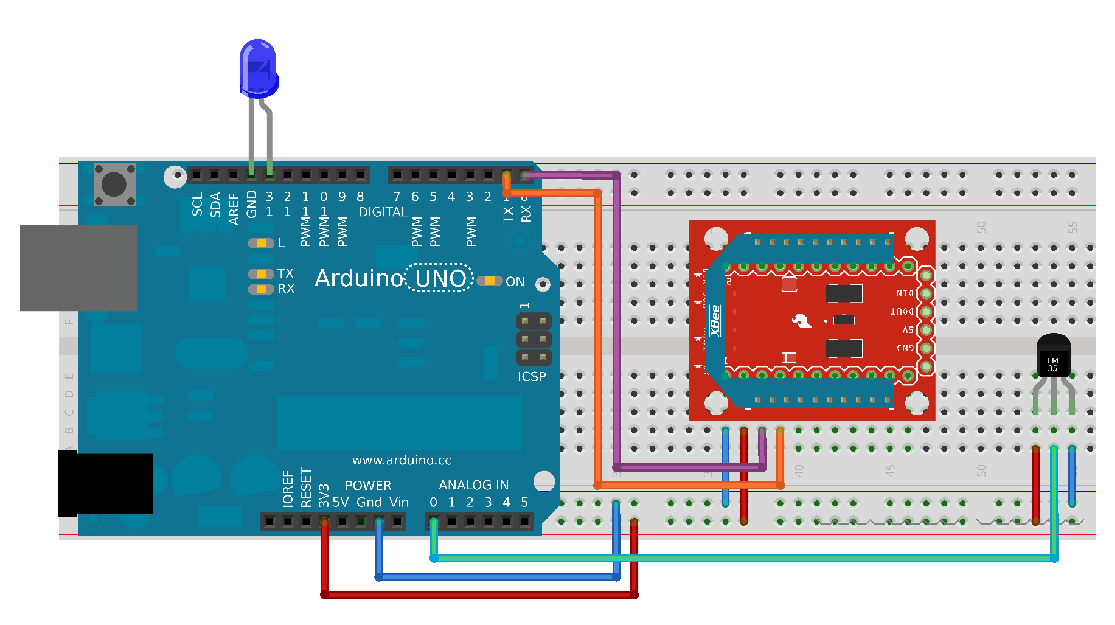
\includegraphics[width=0.85\linewidth]{figures/thermometerInArduino.eps}
  \caption{Thermometer and XBee transmitter.}
  \label{fig:thermometerInArduino}
\end{figure}

Use the example code in Listing \ref{code:ATWSN-router} as a reference to read data from the sensors and send it using the serial connection from the Arduino to the XBee. 
Then the XBee will automatically send it to the remote XBee.
Note that in the code we include identifiers for the node and sensor.

\begin{lstlisting} [caption = {Reading from analog input and sending the data via the XBee.}, language = C, label = {code:ATWSN-router}, numbers = left, escapeinside={@}{@}]
int ledPin = 13;

void setup()
{
  pinMode(ledPin, OUTPUT);
  Serial.begin(9600);
}

void loop()
{
  digitalWrite(ledPin, HIGH);
  delay(1000);
  digitalWrite(ledPin, LOW);
  delay(1000);
  Serial.print("N "); //node
  Serial.print("10 ");
  Serial.print("S "); //sensor
  Serial.print("1 ");
  Serial.print("T ");
  Serial.println(analogRead(A0));
}
\end{lstlisting}


The other XBee will be connected directly to the computer.
This will be the sink and will gather the sensed data.
We will program this part in Python using the Listing \ref{code:ATWSN-sink} for reference.


\begin{lstlisting} [caption = {Simple code that reads the message that arrive to the XBee in AT mode.}, language = Python, label = {code:ATWSN-sink}, numbers = left, escapeinside={@}{@}]

# Derived from code by Alejandro Andreu
import serial
import time
import sys
import shlex
from time import gmtime, strftime

print 'Receiving data in transparent mode'

def main():
    if len(sys.argv) is 1:
        print 'You must provide the path to the serial port as an argument, for instance: "python <code.py> /dev/ttyUSB0".'
        sys.exit()
    portname = sys.argv[1]
    try:
        with open(portname) as f: pass
    except IOError as e:
        print e, '\n'
        sys.exit()

    s = serial.Serial(portname, 9600)

    print 'Opened'

    while 1:
        received = s.readline()
        print "Received at: ", strftime("%d-%m-%Y %H:%M:%S",gmtime()),": ", received
        #splitted = shlex.split(received)
        #for i in range(len(splitted)):
        #    print splitted[i]
        time.sleep(1)

if __name__ == "__main__":
    main()
\end{lstlisting}

Now we can collaborate with other groups to build larger networks and do more interesting stuff.
For example
\begin{itemize}
\item Compute time averages, geographical averages and time-geographical averages.
\item Use EWMA or other filters for time average.
\item Create alarms that use a combination of the data received from different sensors and nodes. 
For example, if the majority of nodes report light and temperature readings, trigger a fire alarm.
\item The alarm can be an LED on the Arduinos.
Use broadcast addresses if you want to reach all the nodes in the PANID.
\end{itemize}

\subsection*{Plotting data in real time}
Is not a rare case wanting to plot sensor data in real time. The following code is a modified version of the one shown in Listing~\ref{code:ATWSN-sink}.

\begin{lstlisting} [caption = {Code that grabs the data from the XBee and writes it in a file.}, language = Python, label = {code:ATWSN-sink-toFile}, numbers = left, escapeinside={@}{@}]
# Derived from code by Alejandro Andreu
import serial
import time
import sys
import shlex
from time import gmtime, strftime

print 'Receiving data in transparent mode'

def main():
    if len(sys.argv) is 1:
        print 'You must provide the path to the serial port as an argument, for instance: "python <code.py> /dev/ttyUSB0".'
        sys.exit()
    portname = sys.argv[1]
    try:
        with open(portname) as f: pass
    except IOError as e:
        print e, '\n'
        sys.exit()

    s = serial.Serial(portname, 9600)

    print 'Opened'

    while 1:
        f=open("log.txt","a")
        received = s.readline()
        print "Received at: ", strftime("%d-%m-%Y %H:%M:%S",gmtime()),": ", received
        splitted = shlex.split(received)
        for i in range(len(splitted)):
            if(splitted[i] == 'T'):
                seconds = int(strftime("%H",gmtime()))*3600 + int(strftime("%M",gmtime()))*60 + int(strftime("%S",gmtime()))
                f.write('{0} {1}\n'.format(seconds,splitted[i+1]))
                #f.write(seconds, ' ' , splitted[i+1]+'\n')
        f.close()
        time.sleep(1)

if __name__ == "__main__":
    main()
\end{lstlisting}

The code shown above writes the incoming data in a file called \texttt{log.txt} with the following format: \texttt{<seconds> <data>}. This way we can use any plotting software - like GNUPlot - to read and plot the incoming data.

If this is your first time using GNUPlot, do not worry. Just grab the following code and write it in a \texttt{<whateverName>.gp} file.

\begin{lstlisting} [caption = {GNUPlot file for plotting real-time data.}, language = GNUPlot, label = {code:ATWSN-sink-gnuplot}, numbers = left, escapeinside={@}{@}]
set xrange[*:*]
set yrange[*:*]
set xlabel "Time"
set ylabel "Sensor data"
plot "log.txt" u 1:2 title "Temperature" with l ls 1 lw 2
pause 1
replot
reread
\end{lstlisting}

Listing~\ref{code:ATWSN-sink-gnuplot} is a script that can be executed issuing the following command: \texttt{gnuplot <nameOfTheScript>.gp}.

Execute both scripts in different terminal windows, Listing~\ref{code:ATWSN-sink-toFile} will receive and write the data in a file, while Listing~\ref{code:ATWSN-sink-gnuplot} plots it in real time.

\subsubsection{Further steps}
\begin{itemize}
 \item Try playing with GNUPlot parameters to make your figures easier to read.
 \item Try to modify the temperature (touching the sensor) and see how the plot also changes.
 \item Note that in the Python code we read the received data until a \texttt{T} is detected. This letter was sent to inform that the following characters are coming from the temperature sensor. Try to incorporate more sensors and build your \emph{protocol} appropriately so the new sensor data can be written to a file.
 \item Can you plot multiple sensors in real time?
\end{itemize}

    \chapter{Sunset Sensor}

In this lab assignment you will create a sunset detector using a light-dependant resistor (LDR).
If there is plenty of light, it means than the Sun is high in the sky.
During the day, the detector will light up a white LED.

In the case of complete darkness, the Sun has already gone.
At night, the detector will light up a blue LED.

The sunset detector will display an alarm (either a red LED or buzzer) for intermediate lighting ranges.

The detector consists of two parts that communicate wirelessly, namely the sensor board and the processing board.
The sensor board contains the LDR and an XBee that takes measures and sends them to the other part.
The processing board contains an XBee to receive the data and an Arduino to process it.
The processing board also contains the alarm (LED, buzzer or both).

Use a resistor in series with the LDR to obtain a range of values readable for the XBee analog input.
Take a sample every 255 ms.

On the processing board, use the API firmware to be able to serially read the values that the remote XBee is sending.
Check which is the received value and if it is in the range of interest (intermediate) activate the alarm (LED or buzzer).

\section{What you need}

\begin{itemize}
\item Breadboard (two better than one).
\item Jumper wire.
\item Arduino UNO (and USB-A-to-B cable)
\item 2 XBee S2.
\item 2 XBee explorer (and at least one USB-to-mini-USB cable)
\item Three LEDs (white, red, blue)
\item A buzzer (optional)
\item A photoresistor (or Light Dependant Resistance). ~10Kohm in the dark, ~1Kohm in bright light.
\item 20Kohm resistor.
\end{itemize}

\begin{figure}[htbp]
  \centering
  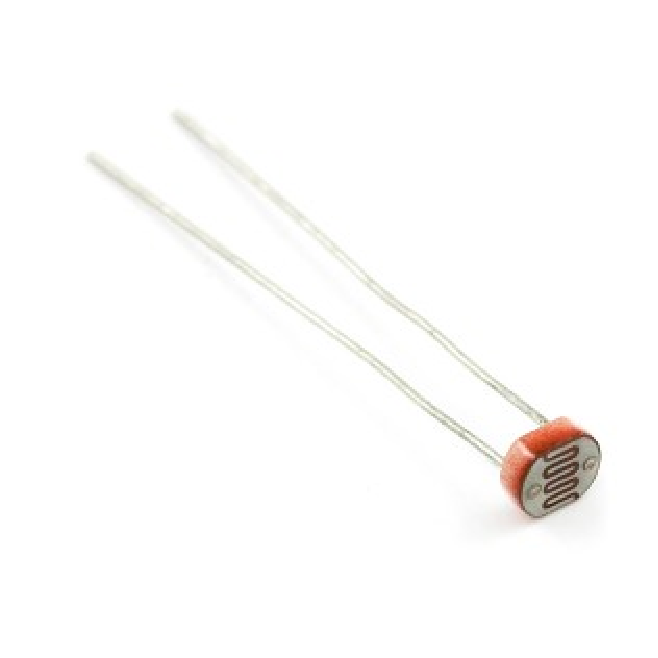
\includegraphics[width=0.3\linewidth]{figures/ldr.eps}
  \caption{LDR}
  \label{fig:blinkingLEDLayout}
\end{figure}

\section{Configuration}
Use X-CTU to configure your XBees.
One of them must be configured as a router (e.g., router AT 22A7 at the time of writing)a and the other as a coordinator API (e.g., coordinator API 21A7 at the time of writing).

For the router, configure the PANID, the destination address (both high and low), enable channel verification (Networking -> JV), set D0 to analog (I/O settings -> D0 -> ADC) and set the sampling rate to 128 ms (I/O settings -> I/O sampling -> IR - I/O sampling rate -> FF).

For the coordinator, you just have to configure the PANID and the destination's address.

\section{Advanced optional assignment}

If you are willing to do more complicated stuff, try to move the alarm to the sensor board. 
Now the sensor board receives the data, sends it to the processing board for processing, and waits for an instruction from the processing board to ring or light the alarm.

    \chapter{Practice: Blink a LED on the XBee from a computer}

In this assignment we will only use two XBees, a protoboard and a LED.
We will not use the Arduino.

Flash the two XBees.
The ``local'' one will be the coordinator and the ``remote'' one, a router.
Use the API mode for the coordinator.
For the remote one, you can use either coordinator, router or end device.
As we are going to interact with the local XBee using the Python library, it is necessary to set the API mode to two (AP=2), as shown in Figure~\ref{fig:changingAPIMode}.

Connect the remote XBee to a protoboard and power it through the USB.
Connect the 5V to the supply voltage bus running along the protoboard.
Finally, connect a LED to bus (long leg) and to the D1 (short leg).

We can blink the remote link by changing the state of the D1 pin from a Python program as in the example code \ref{code:remote-blinking}. Make sure that you have the required XBee Python libraries, available through the link provided in Chapter~\ref{cha:sink-in-server}.\\

\begin{lstlisting} [caption = {This example code alternatively changes a remote pin to up and low to blink an LED.}, language = Python, label = {code:remote-blinking}, numbers = left, escapeinside={@}{@}]

#! /usr/bin/python

from xbee import XBee
import serial
import time

ser = serial.Serial('/dev/ttyUSB0', 9600)
xbee = XBee(ser)

while True:
    try:
        xbee.send('remote_at', 
                  frame_id='A',
                  dest_addr_long='\x00\x00\x00\x00\x00\x00\xFF\xFF',
                  dest_addr='\xFF\xFE',
                  options='\x02',
                  command='D1',
                  parameter='\x05')
          
        time.sleep(1)
        
        xbee.send('remote_at', 
                  frame_id='A',
                  dest_addr_long='\x00\x00\x00\x00\x00\x00\xFF\xFF',
                  dest_addr='\xFF\xFE',
                  options='\x02',
                  command='D1',
                  parameter='\x04')
          
        time.sleep(1)
    except KeyboardInterrupt:
        break

xbee.send('remote_at', 
          frame_id='A',
          dest_addr_long='\x00\x00\x00\x00\x00\x00\xFF\xFF',
          dest_addr='\xFF\xFE',
          options='\x02',
          command='D1',
          parameter='\x05')

ser.close()


\end{lstlisting}

\begin{figure}[htbp]
  \centering
  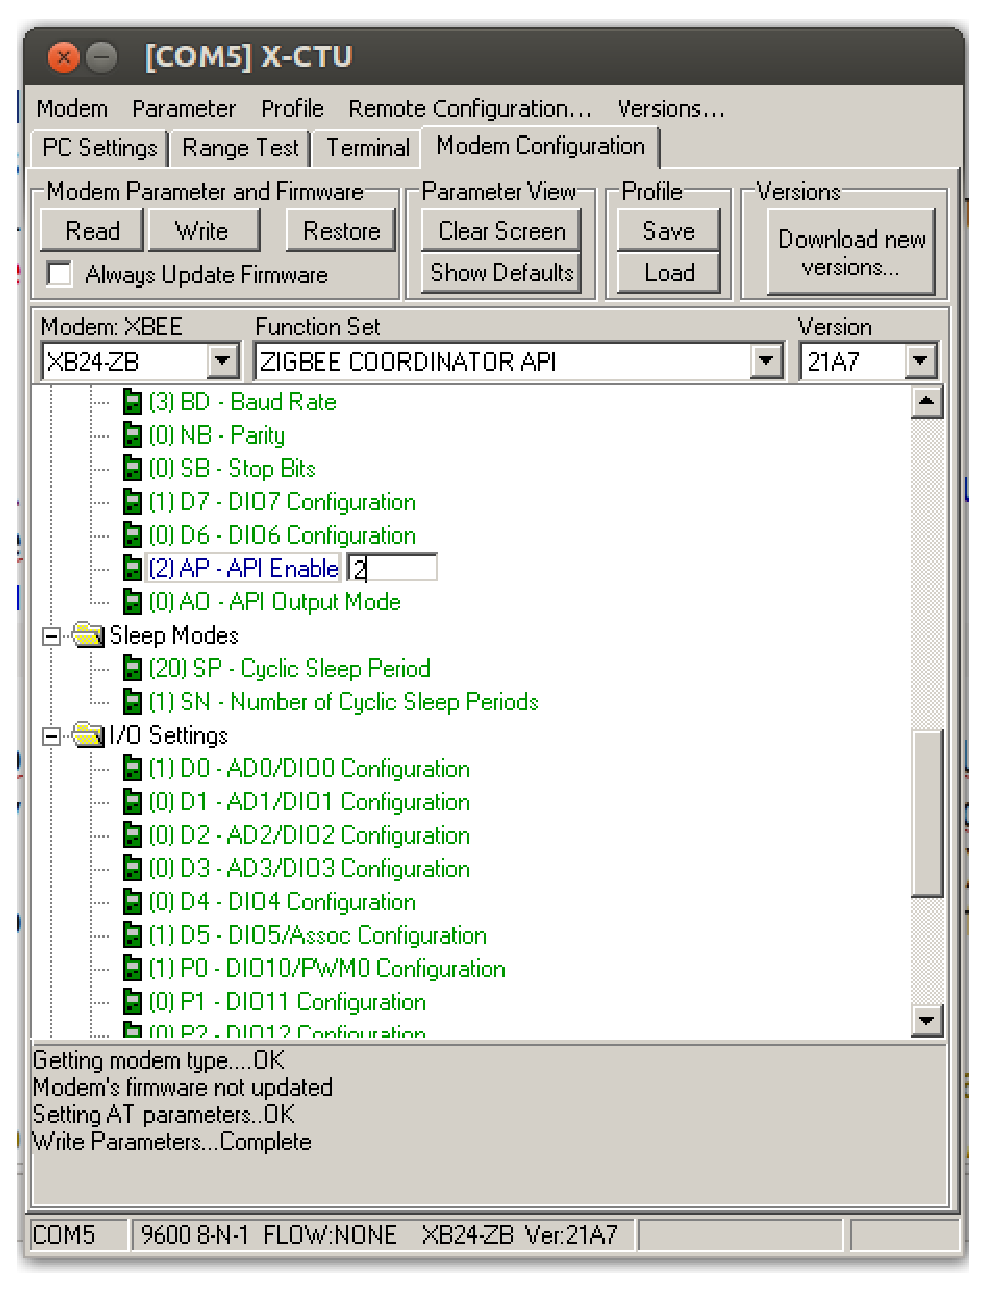
\includegraphics[width=0.85\linewidth]{figures/changingAPIMode.eps}
  \caption{Setting the API mode to 2 (AP=2).}
  \label{fig:changingAPIMode}
\end{figure}

\section{Next steps}
In the example code we use broadcast packets.
Try to blink LEDs in three different XBees alternatively. 
During the first second, the first LED is on.
For the second second, the second LED is on.
And the third LED is on for the third second.
To achieve this you will need to use targeted packets with an explicit destination.

We can also implement the ``sunset sensor'' lab using a computer instead of the arduino.

    \chapter{Sensor Ping}

In this assignment we will implement a ``ping'' over the sensor network.
We will use a script in python to send a probe packet to a remote XBee.
Time is measured between the submission of the packet and the receipt of the acknowledgement and we present the information on the screen to the user.
To makes things more interesting, we connect an Arduino to the remote XBee that flashes a LED each time it receives a packet.
The number of times that the LED has to be flashed is included in the probe packet.

We will start by using X-CTU to flash one of the XBees as a coordinator API and the other as router API.
To prevent interference with other groups, write the PAN ID that you are going to use on the blackboard and make sure that you use a PAN ID different from other groups.
The other XBee should be configured as a Router with the same PAN ID.
It is important to set the API mode to 2 as shown in Fig. \ref{fig:ap2} for the two XBees.
Note that in the computer we are using the ``xbee'' library.


\begin{figure}[htbp]
  \centering
  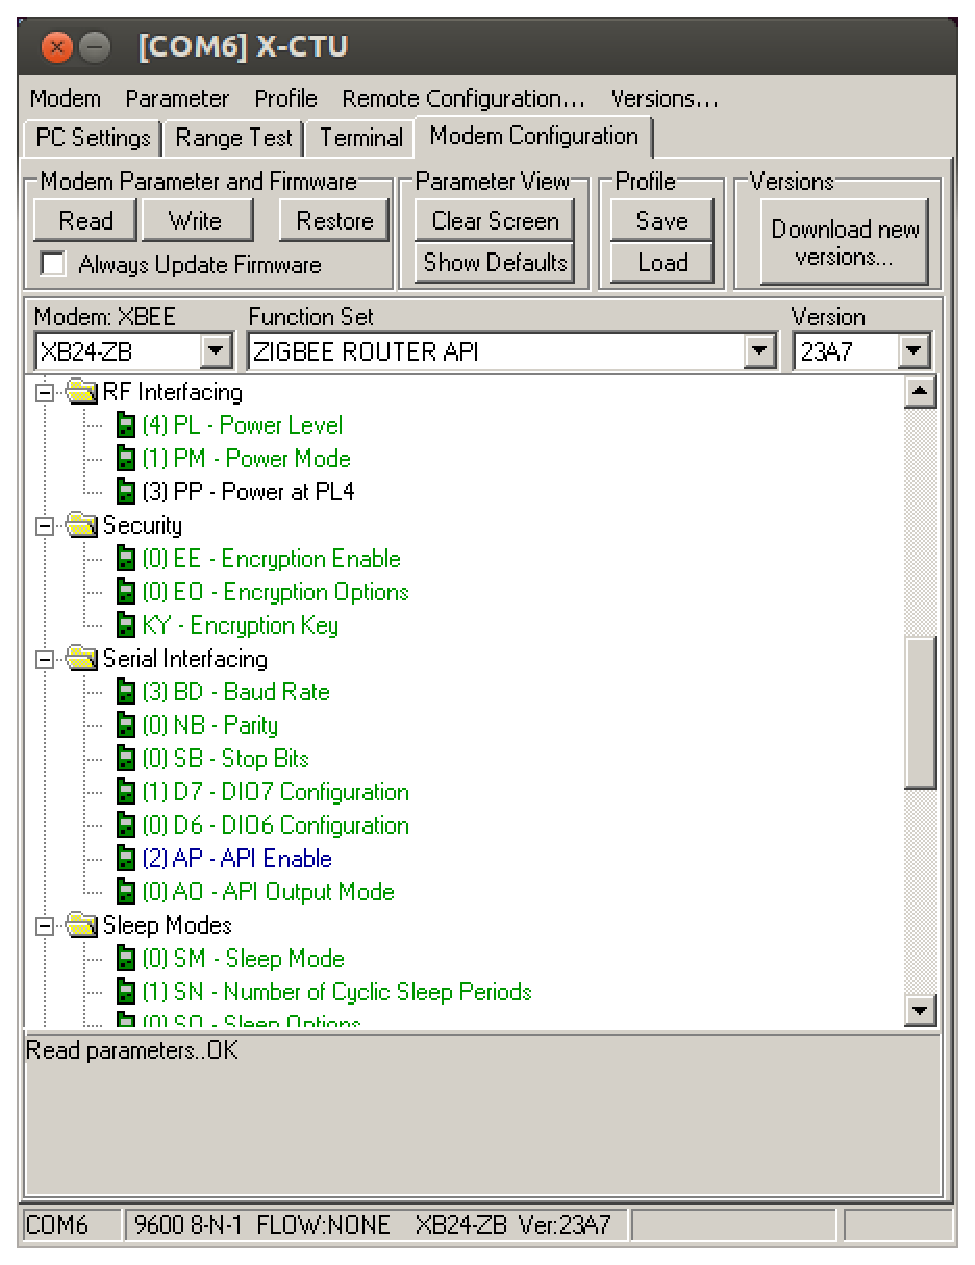
\includegraphics[width=0.9\linewidth]{figures/ap2.eps}
  \caption{Setting the API mode to 2 (AP=2)}
  \label{fig:ap2}
\end{figure}

In the computer, we will create a program that sends a ping packet to the destination every 10s (or whatever you prefer).
Replace the long destination address by the one of your XBee.
Not that the program in listing \ref{code:ping-sender} sends an initial probe packet to obtain the 16-bit address of the destination and then it uses this address for subsequent probes.
The time that elapses from the sending of the probe to the reception of the acknowledgement is the round-trip-time and is printed on the screen.

\begin{lstlisting} [caption = {Simple code that reads the message that arrive to the XBee.}, language = Python, label = {code:ping-sender}, numbers = left, escapeinside={@}{@}]

#! /usr/bin/python

import time
from datetime import datetime
import serial
from xbee import XBee, ZigBee

PORT = '/dev/ttyUSB0'
BAUD_RATE = 9600

# Open serial port and enable flow control
ser = serial.Serial(PORT, BAUD_RATE, bytesize=8, parity='N', stopbits=1, timeout=None, xonxoff=1, rtscts=1, dsrdtr=1)

# Create API object
xbee = ZigBee(ser,escaped=True)

DEST_ADDR_LONG = "\x00\x13\xA2\x00\x40\x8B\x3D\x91"

#part to discovery shot 16-bit address
xbee.send("tx",data="\x01",dest_addr_long=DEST_ADDR_LONG,dest_addr="\xff\xfe")
response = xbee.wait_read_frame()
shot_addr = response["dest_addr"]

# Continuously read and print packets
while True:
    try:
        print "send data"
        tstart = datetime.now()
        xbee.send("tx",data="\x03",dest_addr_long=DEST_ADDR_LONG,dest_addr=shot_addr)
        response = xbee.wait_read_frame()
        tend = datetime.now()
        print tend - tstart
        time.sleep(10)
    except KeyboardInterrupt:
        break

ser.close()

\end{lstlisting}

The provided code should work as soon as you connect the two XBees. 
You can plug the USB cables to power the two XBees and check that everythin is working.
Try to disconnect the remote XBee and observe what happens.

To make thinks more interesting, we will connect an Arduino to the remote XBee and flash a light each time that it receives a packet.
We will use the ``xbee-arduino'' library in the Arduino as explained in the listing 

    \chapter{Collecting data in a computer}

In this assignment we will use some python libraries to receive the data transmitted by the sunset sensor in a computer instead of the Arduino.
You can use one of the university computers, a laptop or a RaspBerry.

Install the XBee python libraries.

\url{http://pypi.python.org/pypi/XBee/2.0.0}

This code offers an implementation of the XBee serial communication API.

We re-use the processing board of the previous assignment and this time we will connect the XBee that receives the data to the computer using the USB cable.
Remember that in the last assignment it was connected to the Arduino.

\begin{lstlisting} [caption = {Simple code that reads the message that arrive to the XBee.}, language = Python, label = {code:simple-receiver}, numbers = left, escapeinside={@}{@}]

import serial
from xbee import ZigBee

print 'Printing data from remote XBee'

serial_port = serial.Serial('/dev/ttyUSB0', 9600)
zigbee = ZigBee(serial_port)

while True:
    try:
        print zigbee.wait_read_frame()
    except KeyboardInterrupt:
        break

serial_port.close()
\end{lstlisting}

You can see the results of running the program in Fig. \ref{fig:sink_in_server_screenshot_first_test}.

\begin{figure}[htbp]
  \centering
  \includegraphics[width=0.9\linewidth]{figures/sink_in_server_screenshot_first_test.eps}
  \caption{A test run of a python program to read the messages that arrive to the XBee.}
  \label{fig:sink_in_server_screenshot_first_test}
\end{figure}

If the processing of each incoming packet takes a long time, the processing must be made asynchronous so that newer packets can be also processed in parallel.
An example of long processing time can be uploading the data to the Internet.

We will define a (callback) function that is called whenever a packet is arrived.
See the listing \ref{code:asynchronous-receiver} for example code.

\begin{lstlisting} [caption = {Simple code that asynchronously reads the message that arrive to the XBee.}, language = Python, label = {code:asynchronous-receiver}, numbers = left, escapeinside={@}{@}]

import serial
import time
from xbee import ZigBee

print 'Asynchronously printing data from remote XBee'

serial_port = serial.Serial('/dev/ttyUSB0', 9600)

def print_data(data):
    """
    This method is called whenever data is received.
    Its only argument is the data within the frame.
    """
    print data['samples']

zigbee = ZigBee(serial_port, callback = print_data)

while True:
    try:
        time.sleep(0.001)
    except KeyboardInterrupt:
        break

zigbee.halt();
serial_port.close()

\end{lstlisting}

You can change the configuration of your router from the coordinator. 
The code snippet in listing \ref{code:sampling-rate}.

\begin{lstlisting} [caption = {Simple code that asynchronously reads the message that arrive to the XBee.}, language = Python, label = {code:sampling-rate}, numbers = left, escapeinside={@}{@}]

zigbee.send('remote_at',
          frame_id='A',
          dest_addr_long='\x00\x13\xa2\x00\x40\x8b\x3d\xe2',
          options='\x02',
          command='IR',
          parameter='\xF2')

\end{lstlisting}

Collaborate with other groups to create larger networks and explore what you can do with the data using python programs (computing averages? sending an email upon a trigger event? dynamically adapting the sampling rate as a function of the measured vales?).


    \chapter{Practice: Sleep}
Flash an XBee with the End-Device AT firmware using X-CTU.
First, plug the XBee in the XBee explorer socket and connect the USB cable.
Use the \texttt{dmesg} command to find to which device is the USB attached.
Look for a line similar to

\texttt{[ 6370.421000] usb 3-2.2: FTDI USB Serial Device converter now attached to ttyUSB0}

The command to invoke X-CTU will be something similar to

\texttt{wine .wine/drive\_c/Program{\textbackslash} Files/Digi/XCTU/X-CTU.exe}

Then set the port as in Fig. \ref{fig:set-port} and test that you can connect to the XBee using the ``Test/Query'' button as in Fig.~\ref{fig:test-xctu}.
\begin{figure}[htbp]
  \centering
  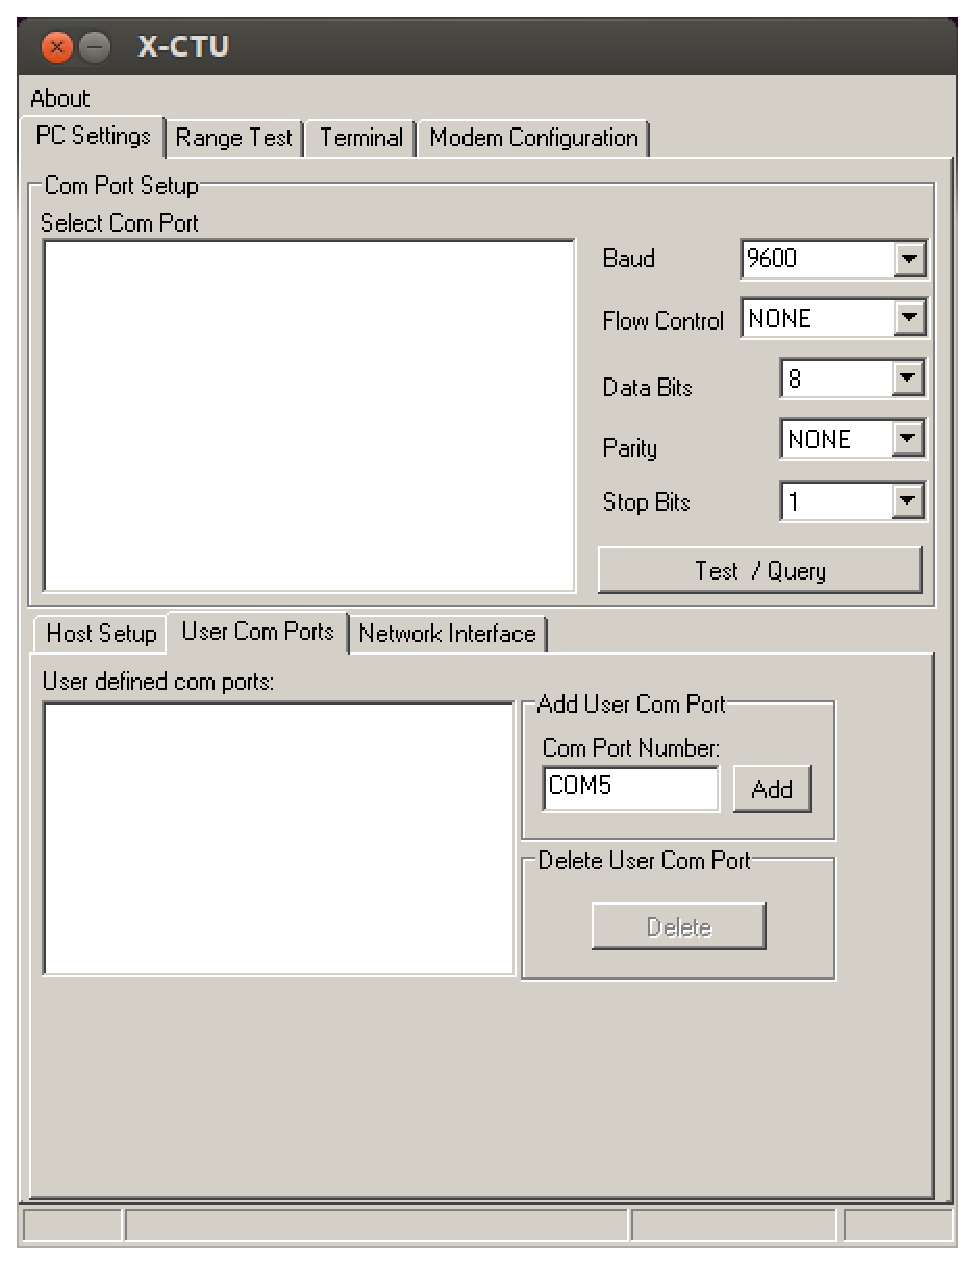
\includegraphics[width=0.3\linewidth]{figures/set-port.eps}
  \caption{Setting the port.}
  \label{fig:set-port}
\end{figure}

\begin{figure}[htbp]
  \centering
  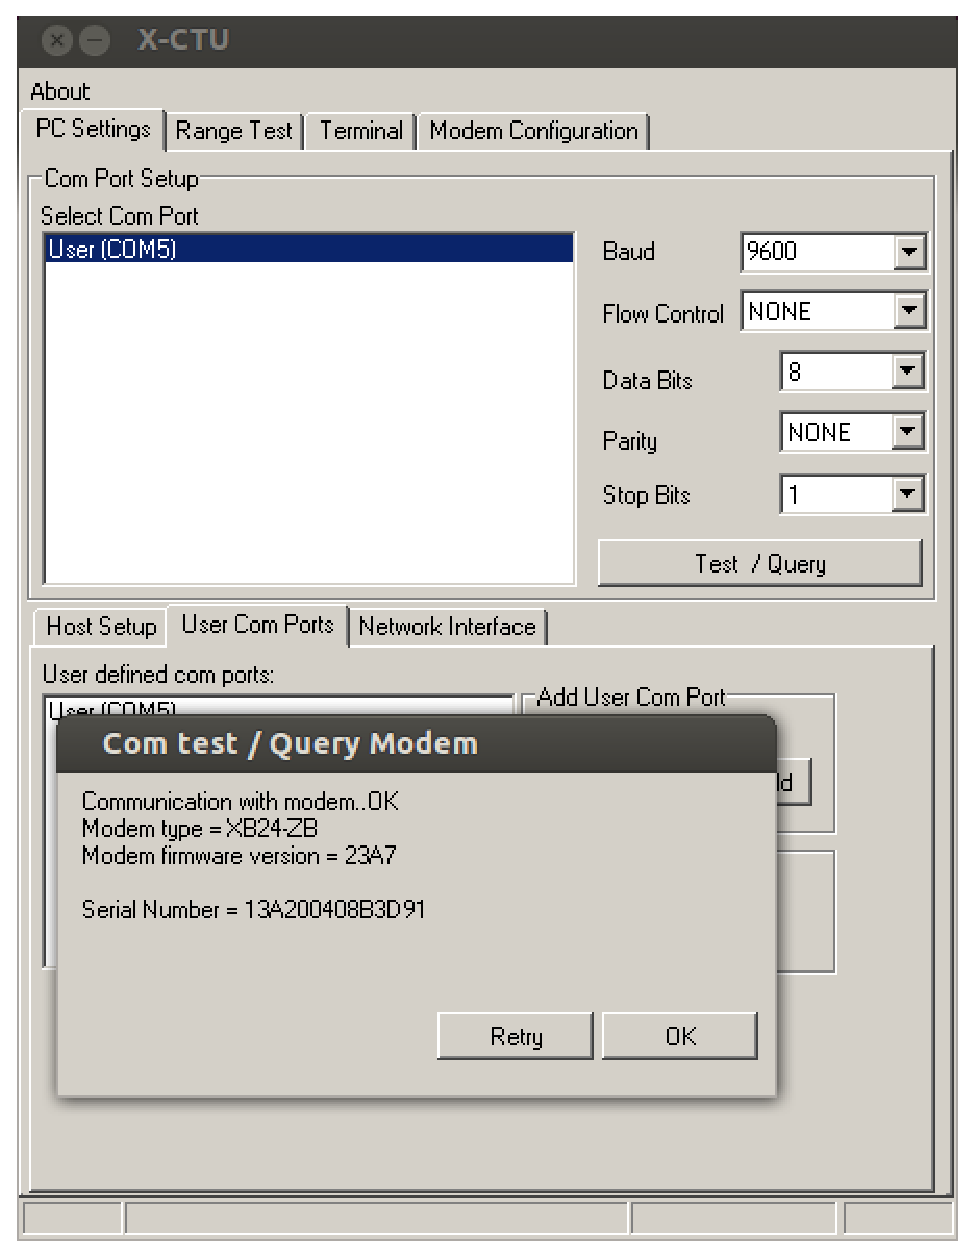
\includegraphics[width=0.3\linewidth]{figures/test-xctu.eps}
  \caption{Testing communication with the XBee.}
  \label{fig:test-xctu}
\end{figure}

Now we switch to the ``Modem Configuration'' tag.
We will flash the XBee with an ``end device'' firmware.
Only end devices can sleep.
Routers and coordinators must be always up.
We choose, for example, the firmware ``zigbee end device at'' in the ``Function set'' drop down menu.
And we write the firmware to the XBee.

Let's also clean all previous configuration.
Click the ``restore'' and ``read'' buttons to restore settings to defaults.
You should obtain something similar to Fig. \ref{fig:clean-28a7}.

\begin{figure}[htbp]
  \centering
  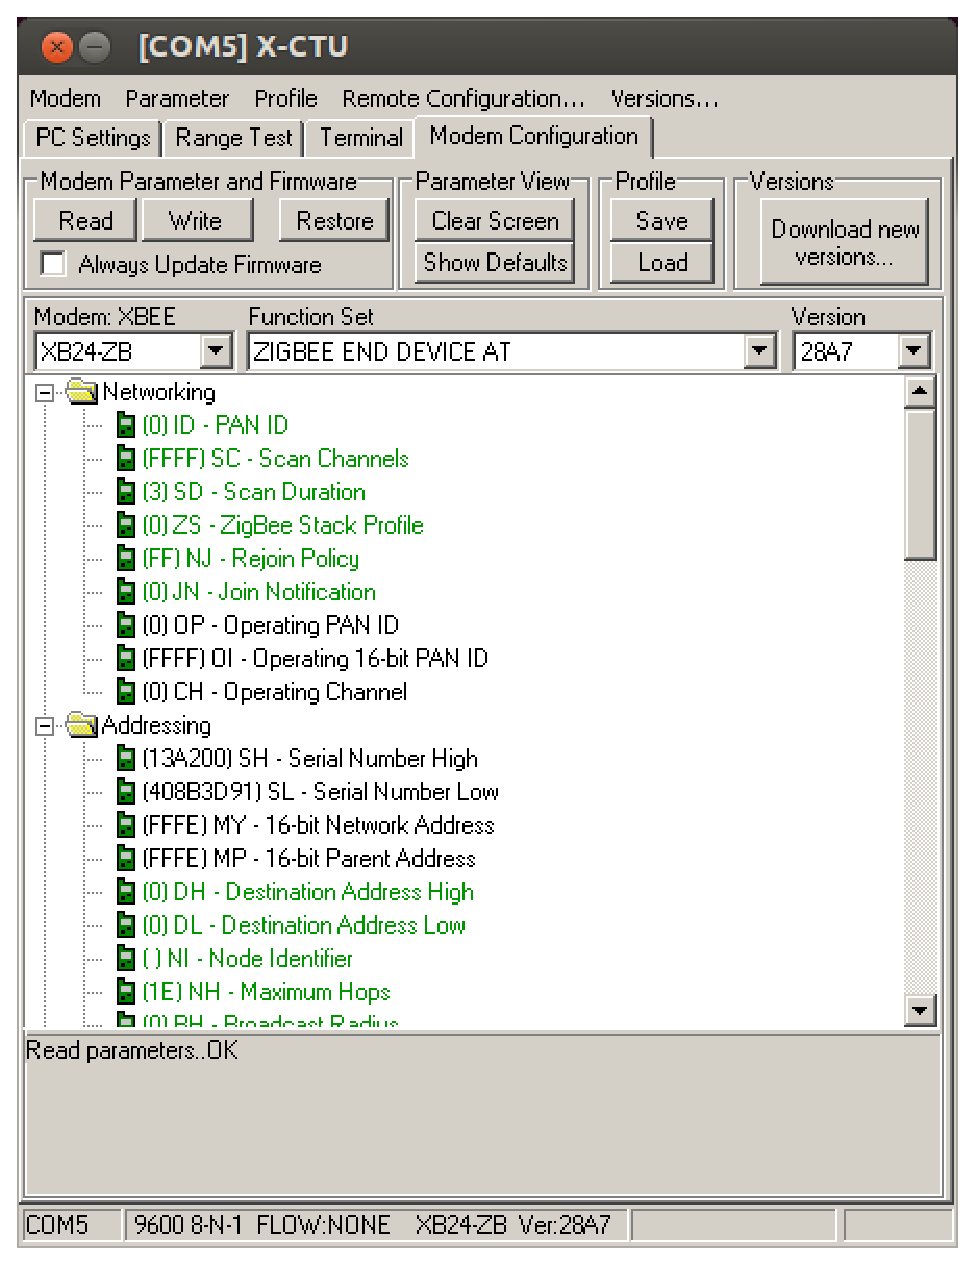
\includegraphics[width=0.3\linewidth]{figures/clean-28a7}
  \caption{Clean 28a7}
  \label{fig:clean-28a7}
\end{figure}

Let's prepare the new configuration.
Set the PAN ID to your group ID.
Set D0 to analog (2).
Set the sampling rate to 255 ms (IR=1FF).
We write the changes to the XBee.
The configuration should look as shown in Fig. \ref{fig:configured-end-device}

\begin{figure}[htbp]
  \centering
  \includegraphics[width=0.3\linewidth]{figures/configured-end-device}
  \caption{Configured end device. D0 set to 2 and IR set to 1FF.}
  \label{fig:configured-end-device}
\end{figure}

Now we need to configure the coordinator just as we configured it for 
Chapter \ref{cha:sink-in-server}.
We write a coordinator API firmware and restore to factory defaults.

We set the PAN ID.
And we write the configuration.

Now run the python program to read incoming data, and we will see as our screens fills with the received data, as in Fig. \ref{fig:received-data}.

\begin{figure}[htbp]
  \centering
  \includegraphics[width=0.3\linewidth]{figures/received-data}
  \caption{Data received by the XBee connected to the computer.}
  \label{fig:received-data}
\end{figure}

We have not sleep much so far.
It's time for a nap.
In the end device, change the ATSM to 5.
This gives us the possibility of waking up the XBee using the DTR pin.
Now we change the SP to 200 (default is 20) and we will see that the XBee takes a nap, then sends a few samples, and then takes a nap again.
Let's set the SP to AAA so that the naps are longer.
You will observe that the naps are fairly long, so we can use the DTR pin to wake the XBee.
We can also wake up the XBee for a round of measures by changing the DTR pin from high to low.

Repeat the lab assignment ``collecting data in a computer'' but this time the sensors will be awake for 1 second and then sleep for 10 seconds.
While the sensor is awake, it will send a sample every 100ms.

Now we will connect an LED between DIO9 and ground to see when the XBee wakes up.
Other ways to know when the XBee wakes up are looking at the RSSI led or the CTS flag in the ``terminal'' tab in X-CTU.

Now for a really long sleeping time, set the sleep options (SO) to 4.
This tells the XBee that, in case of not receiving any packets, it should multiply the sleep time by the value in SN (number of sleep periods).
Set SN also to 4 and save the settings to multiply by 4 the sleep time.

\section{Next Steps}
We can try sleeping in an actuator network.
In this case, we have to set the SP to the parent equal to the longest SP of all the children, to make sure that the parent stores the packets until the children wake up.

    \chapter{Practice: Publishing data in Csosm}

Create a user in \emph{\color{blue}{\href{http://cosm.com}{Cosm.com}}} .
You will receive an email with a pointer to create an API-Key.
Create this key as you will need it to interact with cosm.

\begin{lstlisting} [caption = {Command to create a feed}, language = sh, label = {code:create-feed}, numbers = left, escapeinside={@}{@}]

curl --request POST \
     --data '{"title":"My feed", "version":"1.0.0"}' \
     --header "X-ApiKey: YOUR_API_KEY_HERE" \
     --verbose \
     http://api.cosm.com/v2/feeds

\end{lstlisting}

Use the API Key you obtained in the previous step.
Next edit a JSON file (name it, for example, cosm.json) with the contents detailed in Listing \ref{code:data-json}.

Observe the output as in Fig. \ref{fig:create-feed} and you will observe a feed id (the last number in the Location line).

\begin{figure}[htbp]
  \centering
  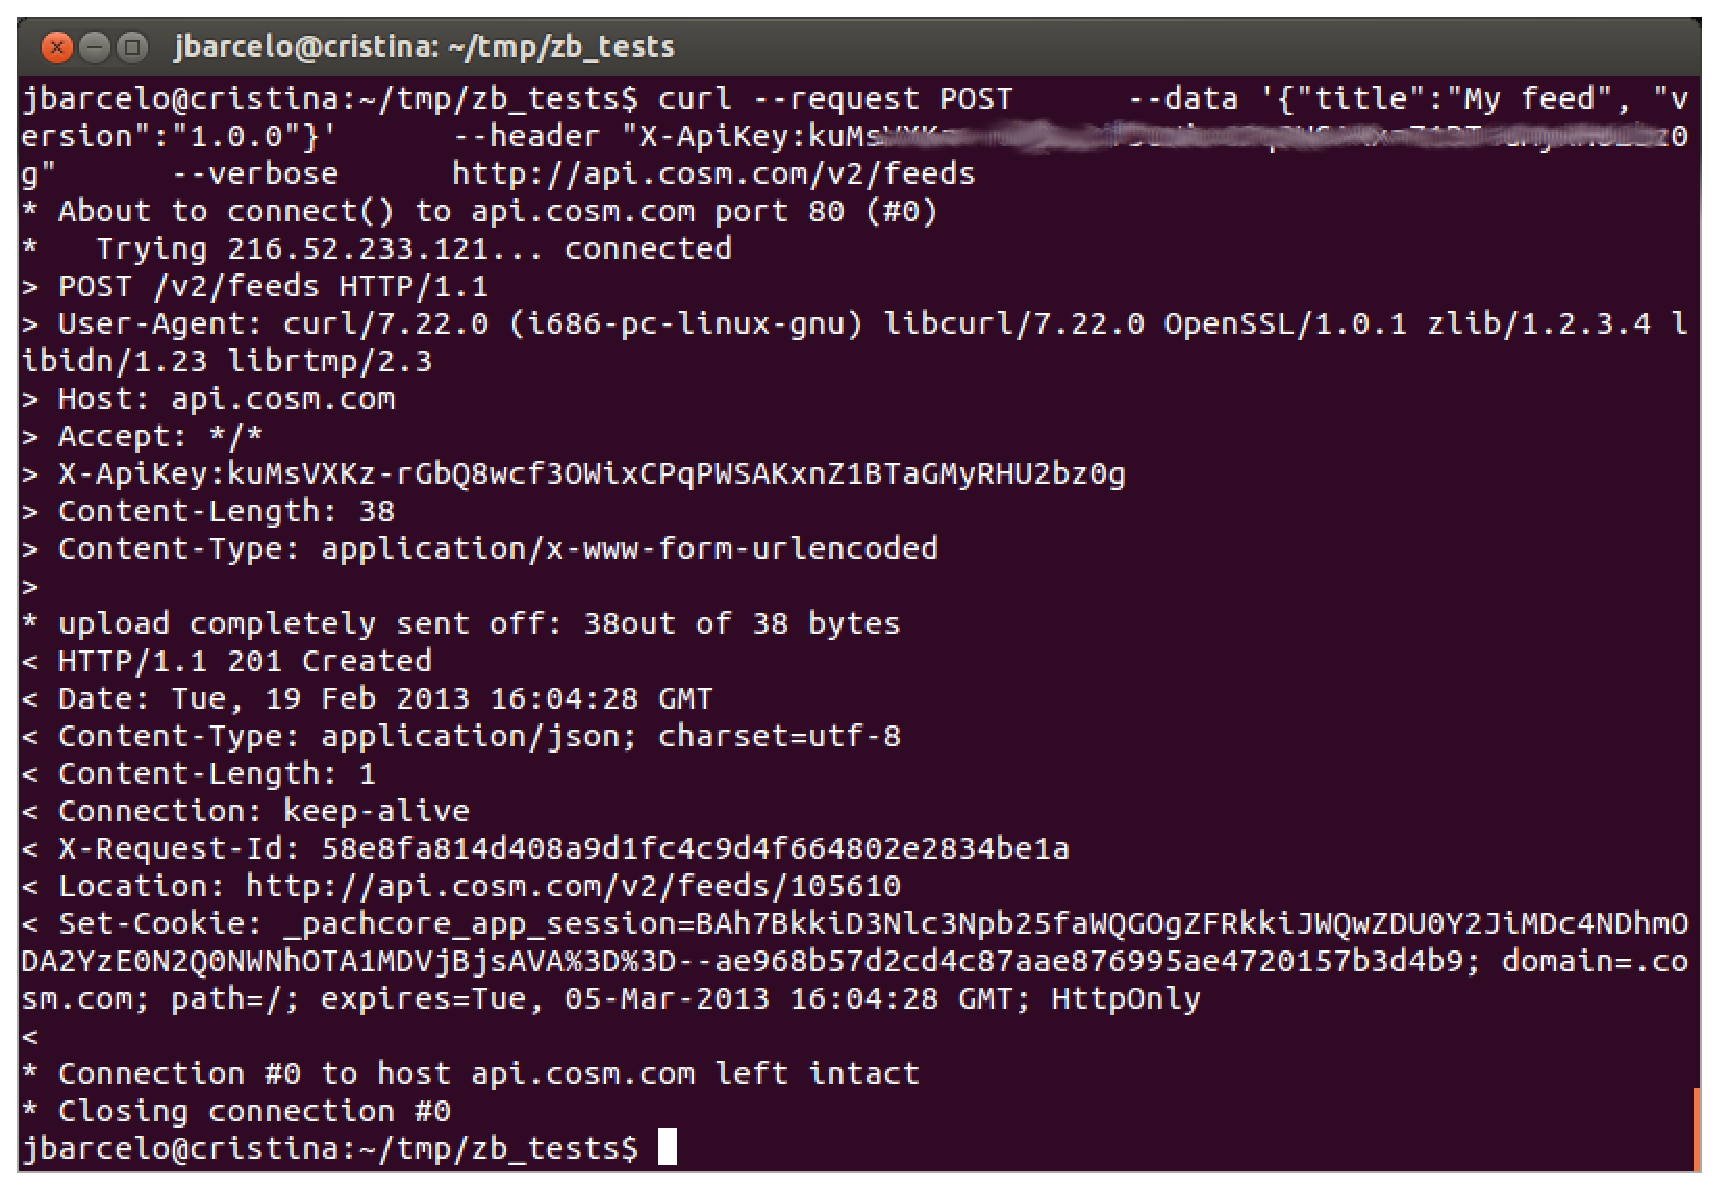
\includegraphics[width=0.9\linewidth]{figures/create-feed.eps}
  \caption{Creating a feed in COSM using curl}
  \label{fig:create-feed}
\end{figure}

Create a JSON file with some dummy data to update to Cosm as in Listing \ref{code:data-json}.

\begin{lstlisting} [caption = {JSON file with data to be uploaded to Cosm}, language = sh, label = {code:data-json}, numbers = left, escapeinside={@}{@}]
{
  "version":"1.0.0",
  "datastreams":[
      {"id":"0", "current_value":"100"},
      {"id":"two", "current_value":"500"},
      {"id":"3.0", "current_value":"300"}
  ]
}
\end{lstlisting}

And now you can update the data to Cosm using the curl command.

\begin{lstlisting} [caption = {Command to upload data to a feed}, language = sh, label = {code:uploading}, numbers = left, escapeinside={@}{@}]
curl --request PUT \
     --data-binary @cosm.json \
     --header "X-ApiKey: YOUR-API-KEY-HERE" \
     --verbose \
     http://api.cosm.com/v2/feeds/YOUR-FEED-ID
\end{lstlisting}

And if we look on Cosm's web interface, we should be able to see some beautiful plots as in Fig. \ref{fig:plots}

\begin{figure}[htbp]
  \centering
  \includegraphics[width=0.9\linewidth]{figures/plots.eps}
  \caption{Plotting data}
  \label{fig:plots}
\end{figure}

You can also read data from the command line as exemplified in Fig. \ref{fig:reading-cosm}.

\begin{figure}[htbp]
  \centering
  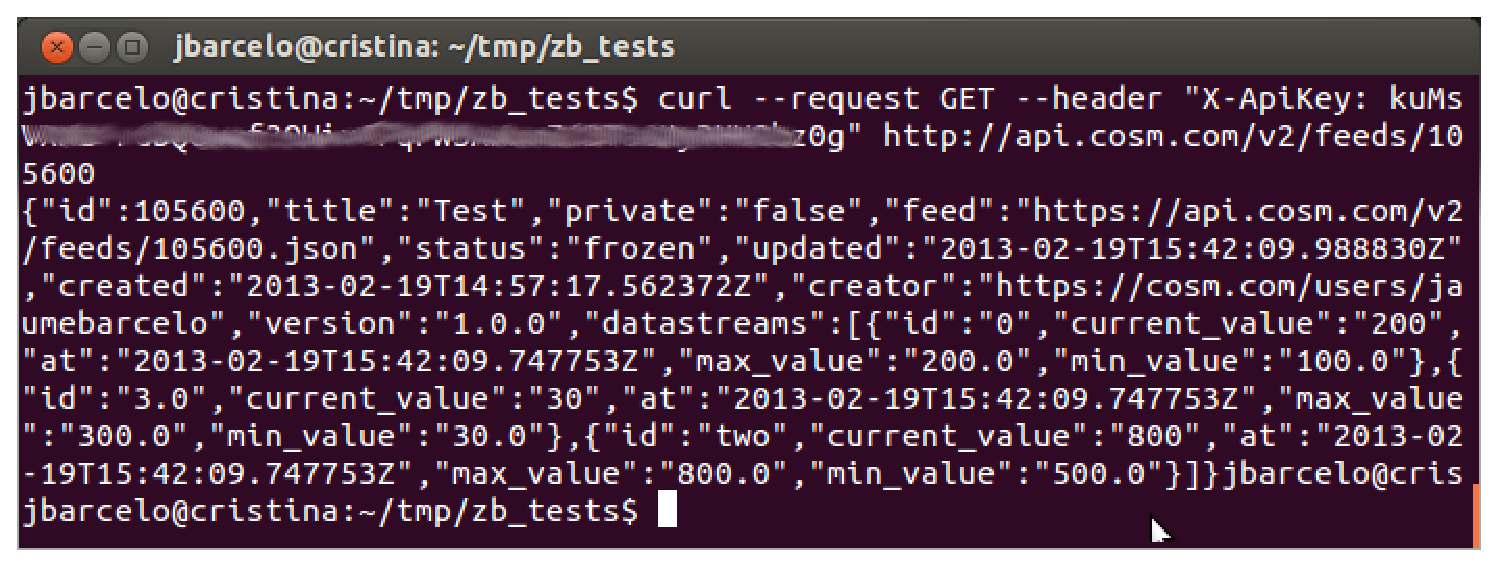
\includegraphics[width=0.9\linewidth]{figures/reading-cosm.eps}
  \caption{Reading a Cosm feed from the command line}
  \label{fig:reading-cosm}
\end{figure}

The next step is to gather information from an XBee and publish it in Cosm.
Use the code detailed in Listing \ref{code:XBee2COSM} as a reference.

\begin{lstlisting} [caption = {Command to upload data to a feed}, language = python, label = {code:XBee2COSM}, numbers = left, escapeinside={@}{@}]
# Derived from code by Alejandro Andreu
import commands
import json
import serial
import time
from serial import SerialException
from xbee import ZigBee

print 'Asynchronously printing data from remote XBee'

serial-port = serial.Serial('/dev/ttyUSB0', 9600)

def print-data(data):
    """
    This method is called whenever data is received.
    Its only argument is the data within the frame.
    """
    print data['samples'][0].keys()[0]

    # Create a JSON file and fill it with the received samples
    json-data = {}
    json-data['version'] = '0.2'
    json-data['datastreams'] = ()
    json-data['datastreams'] = json-data['datastreams'] + ({'id': data['samples'][0].keys()[0], 'current-value': str(data['samples'][0].values()[0])},)
    # Add more datastreams if needed
    with open('cosm.json', mode='w') as f:
        json.dump(json-data, f, indent = 4)
    # Upload information to COSM. Use your own Api Key and feed identifier
    commands.getstatusoutput('curl ... write the curl command here')

zigbee = ZigBee(serial-port, callback = print-data)

time.sleep(1)

zigbee.halt();
serial-port.close()
\end{lstlisting}

Now you can pursue more challenging goals.
For example:
\begin{itemize}
\item Gather information from multiple sensors in a node.
\item Gather information from multiple nodes.
\item Transform the measures of the temperature sensor to Celsius degrees.
\end{itemize}


    \backmatter
%
\bibliographystyle{plain}
\bibliography{my_bib}
\end{document}
